\documentclass{beamer}

\mode<presentation>
{
	\usetheme{Boadilla}
	\setbeamertemplate{navigation symbols}{}
	\setbeamerfont{caption}{size=\scriptsize}
}

\usefonttheme[onlymath]{serif}
\usepackage{mathpazo}

\usepackage{tikz}
\usepackage{amsmath}
\usepackage{bm}
\usepackage{xspace}
\usetikzlibrary{positioning}
\usetikzlibrary{calc}
\usetikzlibrary{shapes.geometric}
% Useful common abbreviations
\newcommand{\adas}{\textsc{adas}\xspace}
\newcommand{\roi}{\textsc{roi}\xspace}
\newcommand{\eg}{e.g.\xspace}
\newcommand{\ekf}{\textsc{ekf}\xspace}

% Useful math
\renewcommand{\H}{\bm{H}}
\newcommand{\rotmat}{\bm{\mathcal{R}}}

% Set path to look for figures
\graphicspath{{fig/}}

% Define title page
\title[Vehicle Tracking with Heading Estimation]{Vehicle Tracking with Heading Estimation \\ using a Mono Camera System}
\subtitle{Master's Thesis at Veoneer}
\author{Fredrik Nilsson}
\institute[]{Performed at the Division of Automatic Control \\ Department of Electrical Engineering \\ Link\"oping University}
\date{\today}

\begin{document}

\begin{frame}
	\titlepage
\end{frame}

\AtBeginSection[]
{
  \begin{frame}{Presentation Outline}
    \tableofcontents[currentsection]
  \end{frame}
}

\begin{frame}{Presentation Outline}
	\tableofcontents
\end{frame}

% -----------------------------------
\section{Introduction}
% -----------------------------------

\begin{frame}{The Traffic Situation in Sweden}
	Important traffic statistic from 2017\footnote{Trafikverket, 2018}
	\begin{itemize}
		\item Average travelled distance per day with car: 30 km
		\item 4400 people were seriously injured
		\item 253 people were killed
	\end{itemize}
	\pause
	\begin{center}
		\large{According to Euro NCAP, 90 \% of all world-wide traffic \\ accidents are caused by the human factor!}
	\end{center}
\end{frame}

\begin{frame}{Euro NCAP}
	The European New Car Assessment Programme
	\begin{itemize}
		\item Performs vehicle tests and rate car models
		\item Vehicle tests of everyday scenarios, \eg
		\begin{itemize}
			\item Automatic emergency braking for vehicles and pedestrians
			\item Adult and child occupant protection
		\end{itemize}
		\item Puts requirements on the car manufacturers
		\item Higher requirements in the near future!
	\end{itemize}
\end{frame}

\begin{frame}{Advanced Driver Assistance Systems (\adas)}
	\begin{columns}
	\column{0.6\textwidth}
	An intelligent system to support and help the driver
	\begin{itemize}
		\item Sensors provide information, \eg
		\begin{itemize}
			\item Camera
			\item Radar
			\item LiDAR
		\end{itemize}
		\item Software to process the data and to make decisions
	\end{itemize}
	Veoneer (spin-off from Autoliv) is a leading supplier for \adas and autonomous driving
	\column{0.35\textwidth}
		\begin{figure}
			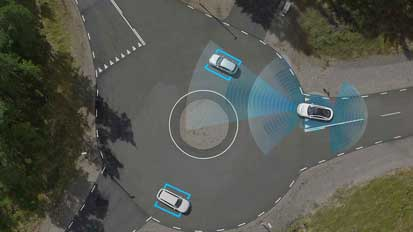
\includegraphics[height=2.25cm]{fig/ALV_Radar-Detection}
			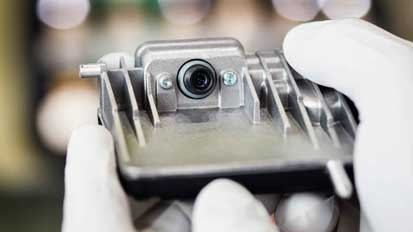
\includegraphics[height=2.25cm]{fig/ALV_Mono-Vision-Sensor}
			\caption{Copyright Autoliv}
		\end{figure}
	\end{columns}
\end{frame}

\begin{frame}{Mono compared to Stereo Vision}
	\begin{columns}
		\column{0.5\textwidth}
		Mono vision
		\begin{itemize}
			\item[$+$] Object detection
			\item[$+$] Less expansive
			\item[$-$] Lacking depth information
			\item[$-$] Increased algorithm complexity
		\end{itemize}
		\column{0.4\textwidth}
		\begin{center}
			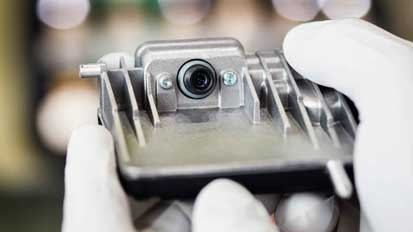
\includegraphics[width=3cm]{fig/ALV_Mono-Vision-Sensor}
		\end{center}
	\end{columns}
	\vspace{1em}
	\begin{columns}
		\column{0.5\textwidth}
		Stereo vision
		\begin{itemize}
			\item[$+$] Object detection
			\item[$+$] Depth information
			\item[$-$] More expensive
		\end{itemize}
		\column{0.4\textwidth}
		\begin{center}
			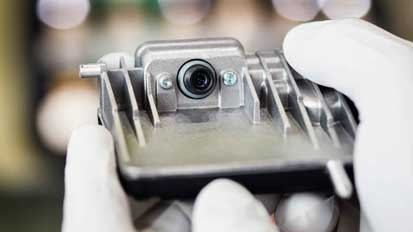
\includegraphics[width=2.25cm]{fig/ALV_Mono-Vision-Sensor}
			\hfill
			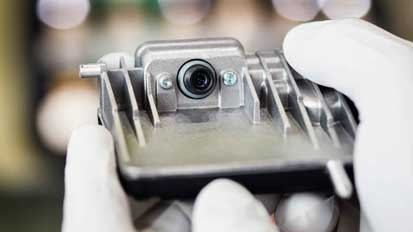
\includegraphics[width=2.25cm]{fig/ALV_Mono-Vision-Sensor}
		\end{center}
	\end{columns}
\end{frame}

\begin{frame}{Objective of the Master's Thesis}
	Since depth information is available in the stereo camera, orientation and angular rate are easy to estimate.
	How can we do that in a mono camera system?
	\pause
	\begin{block}{Objective}
		\begin{itemize}
			\item Can the heading (orientation and angular rate) of a vehicle be estimated using a mono camera system?
			\item Which kind of algorithms and models are suitable for solving the problem?
			\item How does a mono camera system performs compared with a stereo camera system?
		\end{itemize}
	\end{block}
\end{frame}

\begin{frame}{Limitations}
	\begin{itemize}
		\item The algorithm is not required to work in real-time
		\item Perfect knowledge about the ego car's ego motion
		\item Evaluated only on cars
		\item The size of the cars are known
	\end{itemize}
\end{frame}

% ------------------------------
\section{Theory and Methodology}
% ------------------------------

\subsection{Target Tracking}

\begin{frame}{Target Tracking}
	The task of tracking targets:
	\begin{itemize}
		\item Objects of interest
		\item Sensor measurements
		\item Weight measurements with uncertainties
		\item Predict how the objects moves
	\end{itemize}
	Used in for example:
	\begin{itemize}
		\item Radar-based air surveillance
		\item Military missile guidance
		\item \adas
	\end{itemize}
\end{frame}

\begin{frame}{Target Tracking Flow}
	\begin{figure}
	\centering
	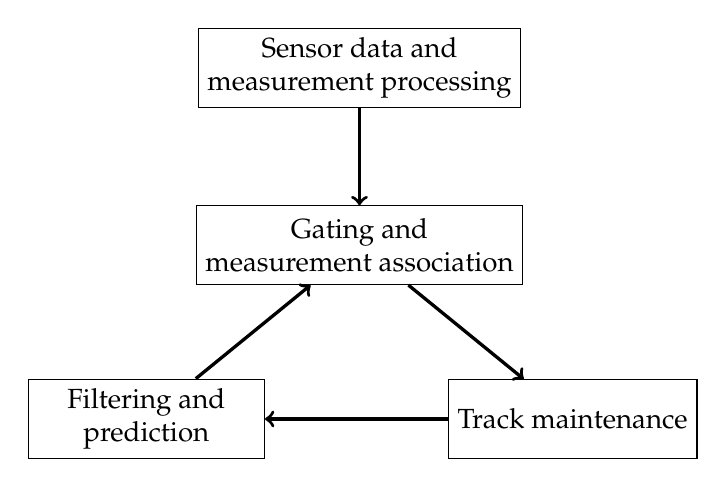
\begin{tikzpicture}
		\tikzstyle{elem} = [rectangle, minimum width = 3cm, minimum height=1cm, align=center, draw=black]

		\node (sensorData) [elem] {Sensor data and \\ measurement processing};
		\node (gatingAssociation) [elem, below of=sensorData, yshift=-1.25cm] {Gating and \\ measurement association};
		\node (trackMaintenance) [elem, below right of=gatingAssociation, yshift=-1.5cm, xshift=2cm] {Track maintenance};
		\node (filter) [elem, below left of=gatingAssociation,  yshift=-1.5cm, xshift=-2cm] {Filtering and \\ prediction};

		\draw [->,very thick] (sensorData) -- (gatingAssociation);
		\draw [->,very thick] (gatingAssociation) -- (trackMaintenance);
		\draw [->,very thick] (trackMaintenance) -- (filter);
		\draw [->,very thick] (filter) -- (gatingAssociation);
	\end{tikzpicture}
	\caption{A flow chart describing a tracking system.}
	\end{figure}
\end{frame}

\begin{frame}{Target Tracking in Mono Vision Systems}
	\begin{columns}[T]
	\column{0.45\textwidth}
	Vehicle detection:
	\begin{itemize}
		\item Appearance-based method
		\item Motion-based method
	\end{itemize}
	\column{0.45\textwidth}
	Vehicle tracking:
	\begin{itemize}
		\item Kalman filter variations
		\item Particle filter
	\end{itemize}
	\end{columns}
	\vfill
	\begin{figure}
		\centering
		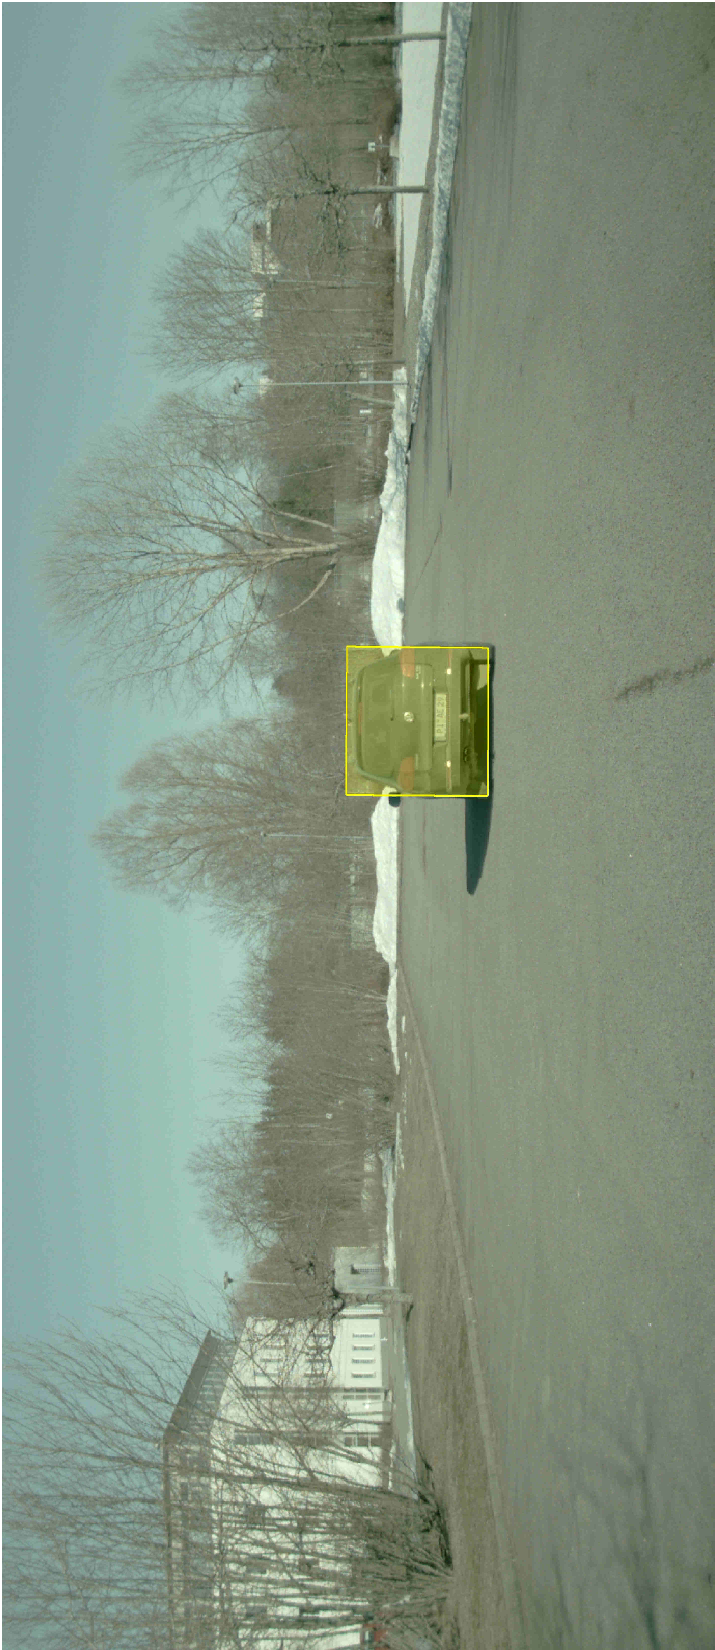
\includegraphics[angle=-90,origin=c,trim={0 0 15cm 0},width=0.6\textwidth]{roi_example}
		\caption{The vehicle has been detected and marked by a box, referred to as the region of interest (\roi).}
	\end{figure}
\end{frame}

\subsection{Feature Points}

\begin{frame}{Feature Points}
	Interesting points in the image.
	\begin{itemize}
		\item Feature detection
		\item Feature description
		\item Feature matching
		\item Feature tracking
	\end{itemize}
	\vfill
	\begin{figure}
		\centering
		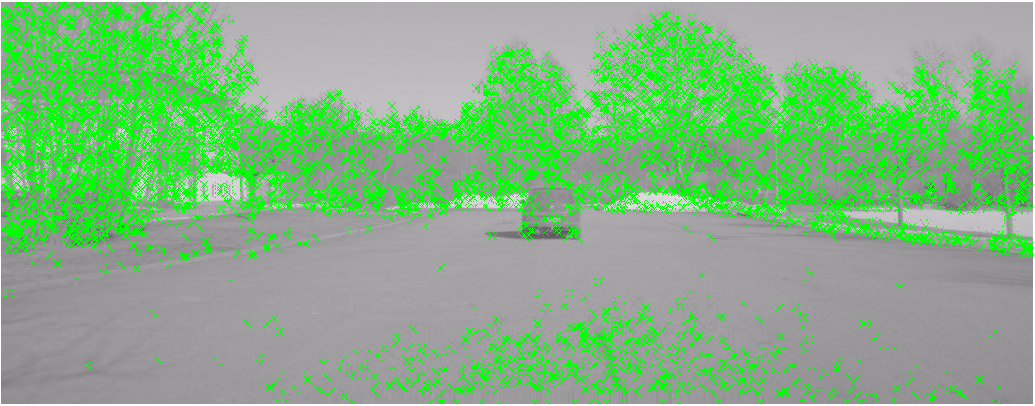
\includegraphics[width=0.6\textwidth]{harris_features}
		\caption{\label{fig:featurepointexample} Detected feature points marked as green crosses.}
	\end{figure}
\end{frame}

\subsection{Projective Transformation}

\begin{frame}{Projective Transformation}
	Mapping between different views of the same planar surface,
	\begin{equation*}
		\bm{x}^\prime \sim \H \bm{x},
	\end{equation*}
	where $\H$ is a nonsingular $3 \times 3$ matrix.
	\vspace{1em}
	The \textit{homography} $\H$ can be decomposed into
	\begin{equation*}
		\H = \rotmat + \bm{t} \bm{n}^T.
	\end{equation*}
\end{frame}

\begin{frame}{The Homography -- A Geometrical View}
	\begin{figure}
		\centering
		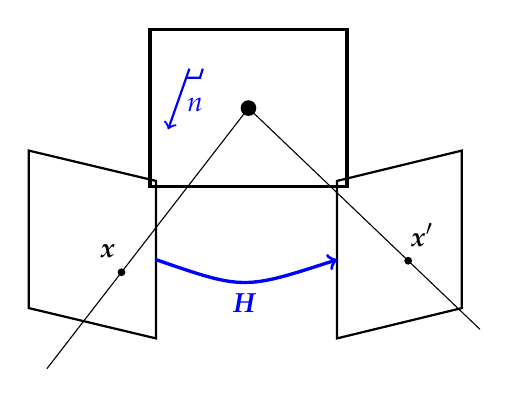
\begin{tikzpicture}
			[plane/.style={very thick,black},
			 image/.style={thick,black},
			 line/.style={black}]

			\draw[plane] (0,0,0) rectangle (2.5,2,0);
			\draw[thick,->,blue] (0.5,1.5,0) -- (1,1.5,2) node[pos=0.6,anchor=west] {$n$};
			\draw[thick,blue] (0.67,1.5,0) -- (0.75,1.5,0.3) -- (0.58,1.5,0.3);

			\draw[image] (0,0,4) -- (0,2,4) -- (2,2,5) -- (2,0,5) -- cycle;
			\draw[image] (4.3,0,5) -- (4.3,2,5) -- (5.5,2,4) -- (5.5,0,4) -- cycle;

			\draw[line] (1.25,1,0) node[circle,fill,inner sep=2pt] {} -- node[label={\hspace{-1em}$\bm{x}$},pos=0.63,circle,fill,inner sep=1pt] {} (1,0,6);
			\draw[line] (1.25,1,0) -- node[label={\hspace{1em}$\bm{x}^\prime$},pos=0.69,circle,fill,inner sep=1pt] {} (6.5,0.5,6);

			\draw[very thick,->,blue] (2,1,5) .. controls (3.5,1,6) .. (4.3,1,5) node[pos=0.5,anchor=north] {$\H$};
		\end{tikzpicture}
		\caption{The homography describing the projective transformation between two views.}
	\end{figure}
\end{frame}

\begin{frame}{Homography for Vehicle Angular Rate}
	\begin{itemize}
		\item Track feature points inside the \roi
		\item Find the homography between consecutive frames
		\item Decompose and extract the yaw rotation
		\item Calculate the angular rate
	\end{itemize}
	\begin{figure}
		\centering
		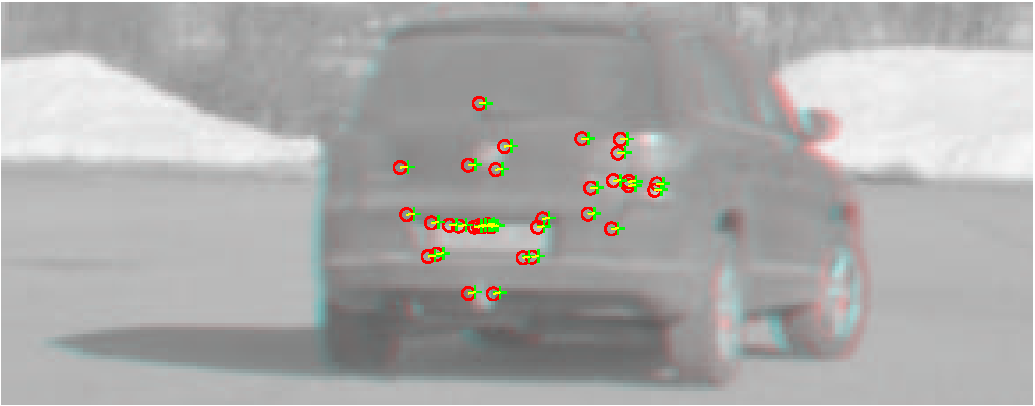
\includegraphics[width=0.8\textwidth]{feature_point_correspondence}
		\caption{Here, feature points have moved from the $1^\text{st}$ frame (red circles) to the $2^\text{nd}$ frame (green crosses).}
	\end{figure}
\end{frame}

\subsection{Filtering Structure}

\begin{frame}{Filtering Structure}
	\begin{figure}
		\centering
		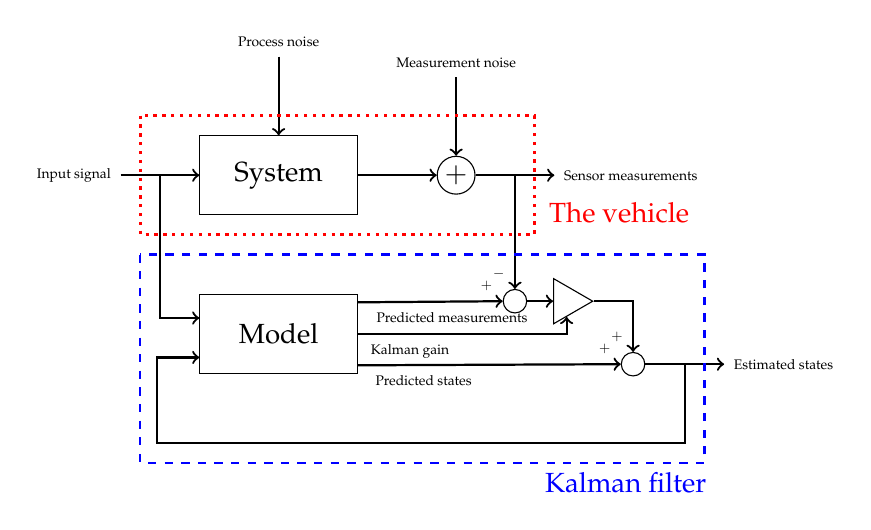
\begin{tikzpicture}
			\tikzstyle{box} = [rectangle, minimum width=2cm, minimum height=1cm, align=center, draw=black]
			\tikzstyle{triangle} = [regular polygon, regular polygon sides=3, align=center, draw=black, shape border rotate=-90]
			\tikzstyle{line} = [thick, black]
			\tikzstyle{sum} = [circle, draw=black, inner sep=1pt]
			\tikzstyle{comb} = [circle, draw=black, inner sep=3pt]

			\node (system)  [box] {System};
			\node (model) [box, below=of system)] {Model};
			\node (sumMeasNoise) [sum, right=of system] {$+$};
			\node (measNoise) [above=of sumMeasNoise] {\tiny Measurement noise};
			\node (procNoise) [above=of system] {\tiny Process noise};
			\node (inputSignal) [left=of system] {\tiny Input signal};
			\node (outputSignal) [right=of sumMeasNoise] {\tiny Sensor measurements};
			\node (combMeas) [comb] at ($(outputSignal.west)+(-0.5,-1.6)$) {};
			\node (combInov) [comb] at ($(combMeas)+(1.5,-0.8)$) {};
			\node (gain) [triangle] at ($(combMeas.east)+(0.5,0)$) {};
			\node (filterOutput) [right=of combInov] {\tiny Estimated states};

			% The system
			\draw[line,->] (procNoise) -- (system);
			\draw[line,->] (inputSignal) -- (system);
			\draw[line,->] (system) -- (sumMeasNoise);
			\draw[line,->] (measNoise) -- (sumMeasNoise);
			\draw[line,->] (sumMeasNoise) -- (outputSignal);

			% The filter
			\onslide<1>
			{
				\draw[line,->] ($(inputSignal.east)+(0.5,0)$) |- ([yshift=0.3cm]model);
			}
			\draw[line,->] ([yshift=0.4cm]model.east) -- (combMeas.west) node[pos=0.65, anchor=north] {\tiny Predicted measurements} node[anchor=south east] {\tiny $+$};
			\draw[line,->] ($(outputSignal.west)+(-0.5,0)$) -- ($(outputSignal.west)+(-0.5,-0.75)$) -| (combMeas.north) node[anchor=south east] {\tiny $-$};
			\draw[line,->] (combMeas.east) -- (gain);
			\draw[line,->] ([yshift=-0.0cm]model.east) -| (gain.south)  node[pos=0.125, anchor=north] {\tiny Kalman gain};
			\draw[line,->] (gain.east) -| (combInov.north) node[anchor=south east] {\tiny $+$};
			\draw[line,->] ([yshift=-0.4cm]model.east) -- (combInov.west) node[pos=0.25, anchor=north] {\tiny Predicted states} node[anchor=south east] {\tiny $+$};
			\draw[line,->] (combInov) -- (filterOutput);
			\draw[line,->] ([xshift=-0.5cm]filterOutput.west) -- ($(filterOutput.west)+(-0.5,-1)$) -- ($(filterOutput.west)+(-7.2,-1)$) |- ([yshift=-0.3cm]model.west);

			\onslide<2>
			{
			% Surround the filter with a box
			\draw[thick, dashed, blue] ($(model.north west)+(-0.75,0.5)$) rectangle ($([xshift=-0.5cm]filterOutput.west)+(0.25,-1.25)$) node[yshift=-0.25cm,xshift=-1cm] {Kalman filter};
			% Surround the system with a box
			\draw[very thick, dotted, red] ($(system.north west)+(-0.75,0.25)$) rectangle ($([xshift=-0.5cm]outputSignal.west)+(0.25,-0.75)$) node[anchor=south east,xshift=2.1cm] {The vehicle};
			}
		\end{tikzpicture}
	\end{figure}
\end{frame}

\begin{frame}{Different Image Measurements}
	\begin{columns}
	\column{0.45\textwidth}
	\begin{tikzpicture}
		\node[] at (0,0) {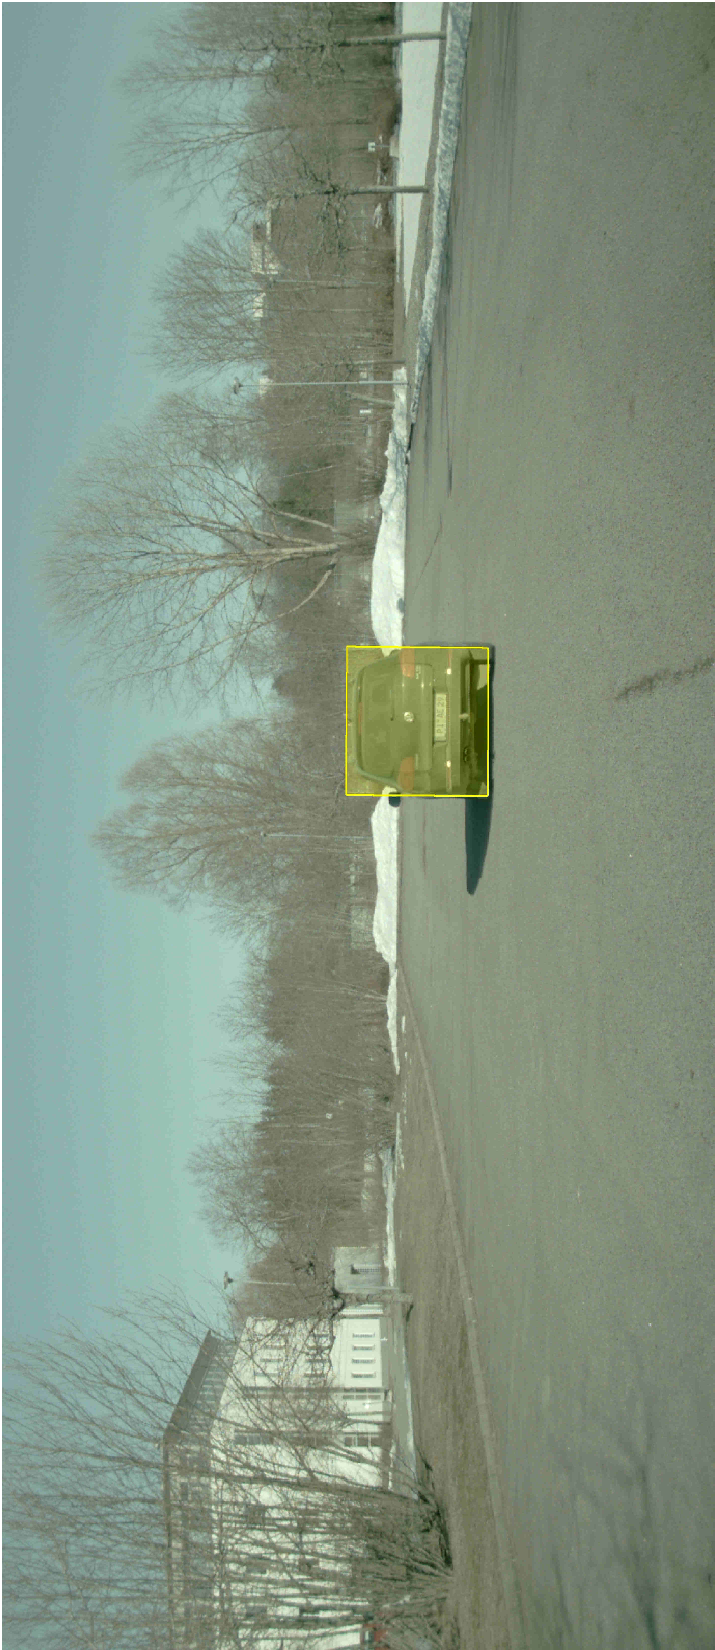
\includegraphics[angle=-90,origin=c,trim={0 0 15cm 0},width=\textwidth]{roi_example}};
		\draw[red, thick, |->] (0,-0.4) -- (0.35,-0.4) node[anchor=north] {\tiny $p_\text{HCP}$};
	\end{tikzpicture}
	\begin{tikzpicture}
		\node[] at (0,0) {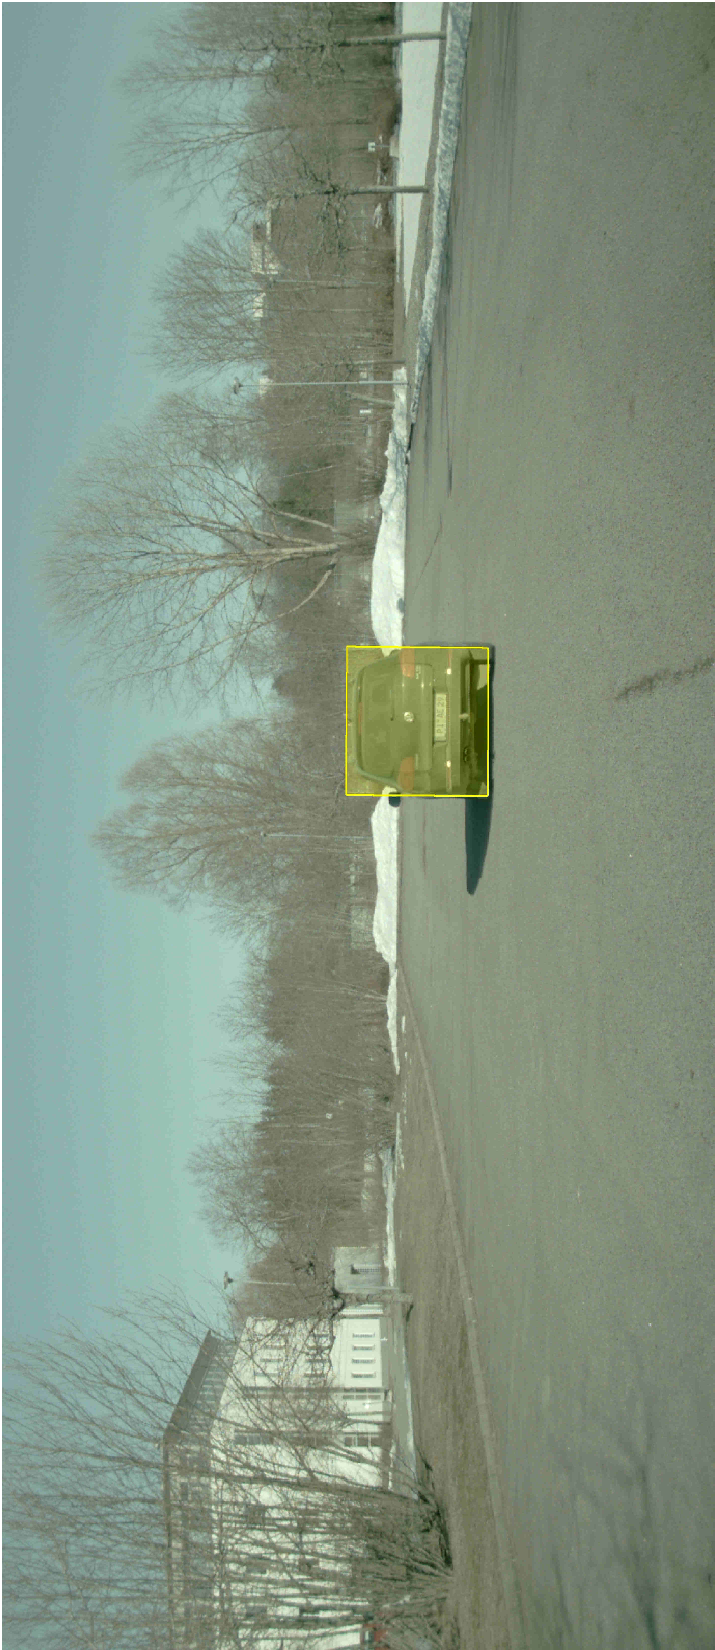
\includegraphics[angle=-90,origin=c,trim={0 0 15cm 0},width=\textwidth]{roi_example}};
		\draw[red, thick, <->] (0.08,0.1) -- (0.6,0.1) node[pos = 0.5, anchor=south] {\tiny $p_\text{Width}$};
	\end{tikzpicture}
	\column{0.45\textwidth}
	\begin{tikzpicture}
		\node[] at (0,0) {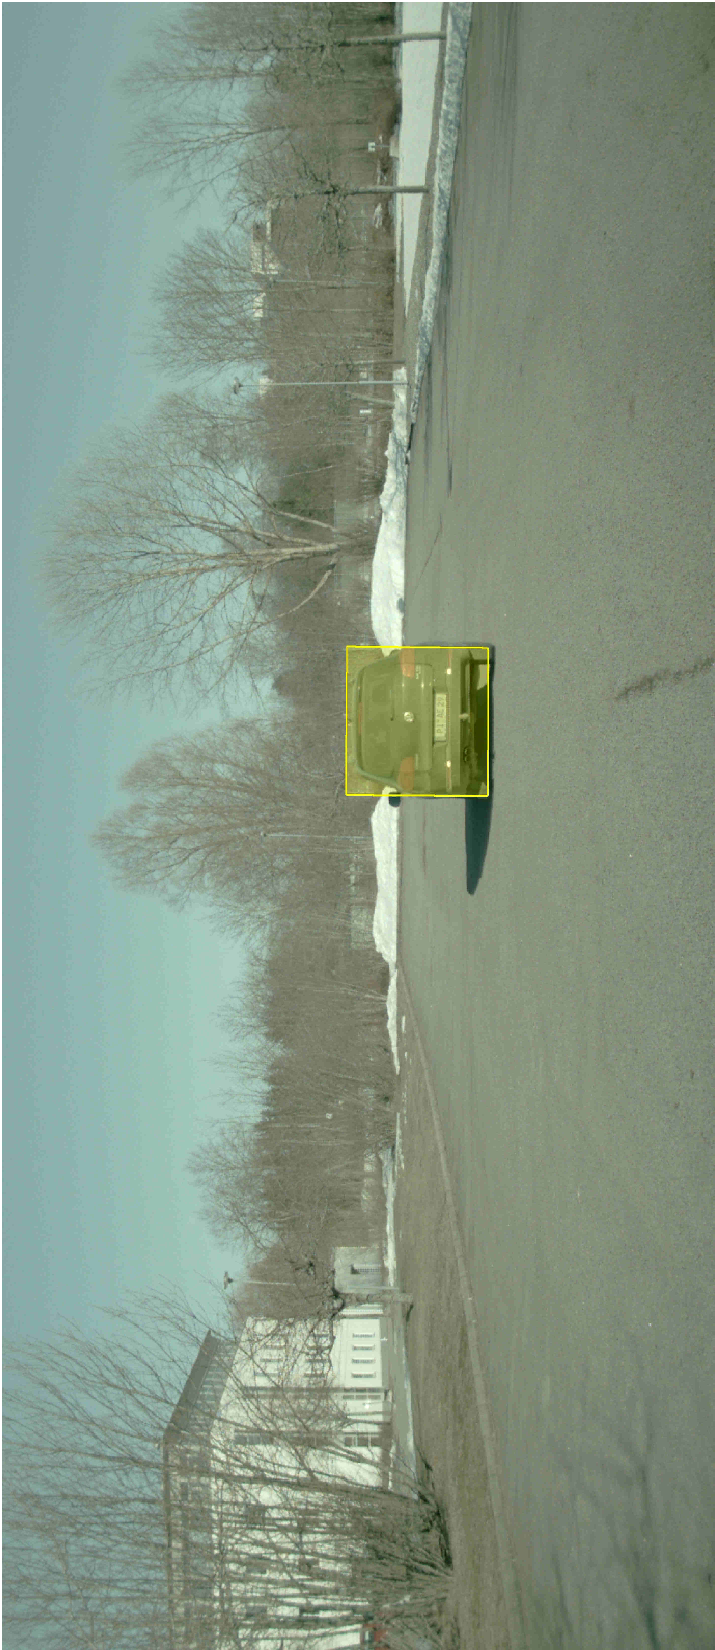
\includegraphics[angle=-90,origin=c,trim={0 0 15cm 0},width=\textwidth]{roi_example}};
		\draw[red, thick, |->] (0.35,0) -- (0.35,-0.38) node[pos = 0.5, anchor=west] {\tiny $p_\text{Bottom}$};
	\end{tikzpicture}
	\begin{tikzpicture}
		\node[] at (0,0) {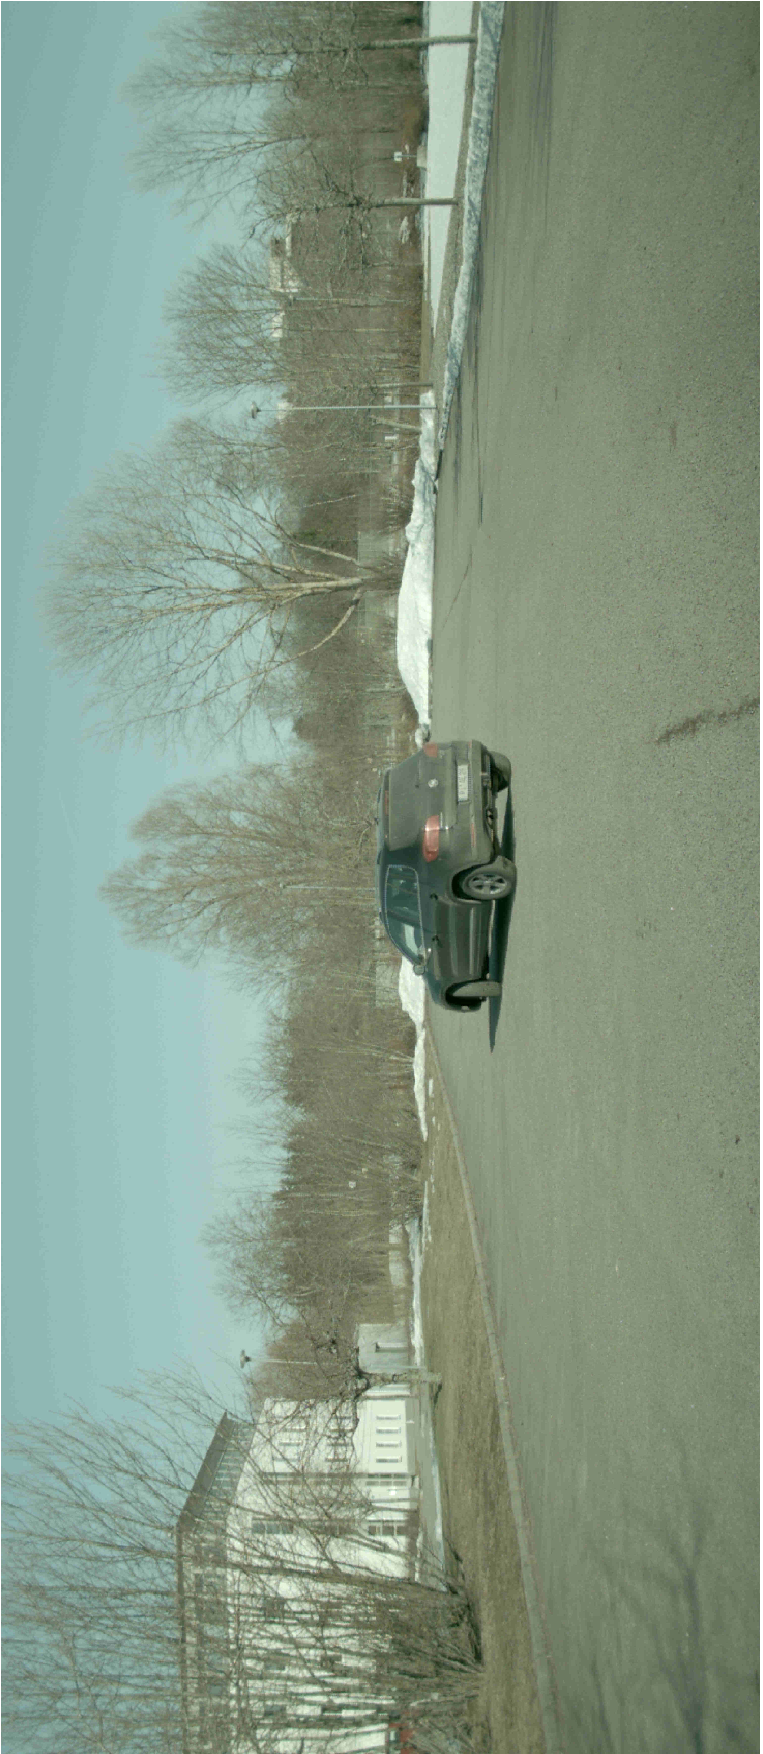
\includegraphics[angle=-90,origin=c,trim={0 0 16cm 0},width=\textwidth]{corners_example}};
		\node[red,circle,fill,inner sep=0.5pt,label=left:{\color{red}\tiny FL}] at (-0.4,-0.35) {};
		\node[red,circle,fill,inner sep=0.5pt,label=below:{\color{red}\tiny RL}] at (0.075,-0.4) {};
		\node[red,circle,fill,inner sep=0.5pt,label=right:{\color{red}\tiny RR}] at (0.4,-0.37) {};
	\end{tikzpicture}
	\end{columns}
\end{frame}

\begin{frame}{Summary of the Filter Structure}
	\begin{columns}
	\column{0.6\textwidth}
		\begin{itemize}
			\item Vehicle modelled as a rectangle
			\item An extended Kalman filter (\ekf)
			\item A constant velocity motion model
			\item State vector $\bm{x}=\begin{pmatrix} x & y & z & v & \psi & \omega \end{pmatrix}^T$
		\end{itemize}
	\column{0.4\textwidth}
		\begin{figure}
			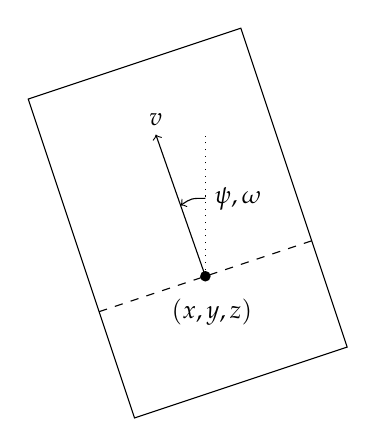
\begin{tikzpicture}[scale=0.9, every node/.style={scale=0.9}]
				\draw (0,0) -- (3,1) -- (1.5,5.5) -- (-1.5,4.5) -- cycle;
				\draw[dashed] (-0.5,1.5) -- (2.5,2.5) node[pos=0.3, anchor=north west] {$(x,y,z)$};
				\draw[->] (1,2) node[circle,fill,inner sep=1.5pt] {} -- (0.3,4) node[anchor=south] {$v$};
				\draw[dotted] (1,2) -- (1,4);
				\draw[<-] (0.65,3) .. controls (0.8,3.1) .. (1,3.1) node[pos=0.5, anchor=west] {\hspace{0.2cm}$\psi, \omega$};
		    \end{tikzpicture}
		    \caption{Target vehicle model.}
		\end{figure}
	\end{columns}
\end{frame}

% ---------------
\section{Results}
% ---------------

\subsection{Simulated results}

\begin{frame}{Monte Carlo Simulations -- No. 1}
	The target is driving straight.
	\vspace{2em}
	\begin{columns}
	\column{0.45\textwidth}
	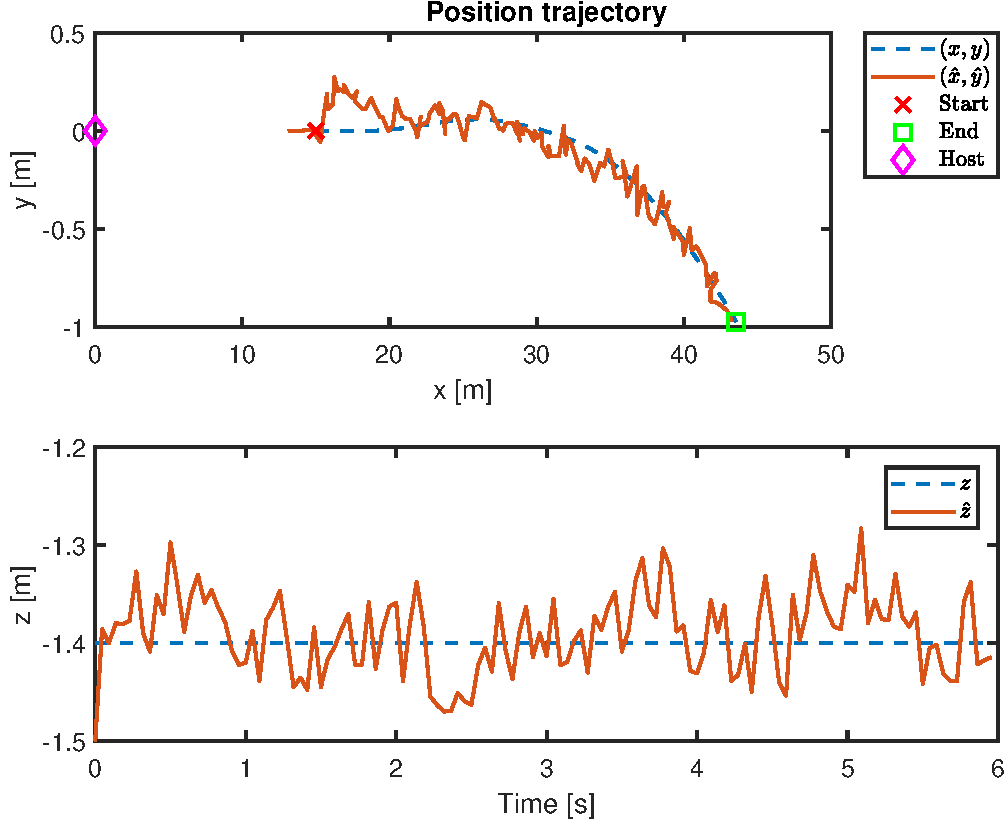
\includegraphics[width=\textwidth]{Traj/20_MC_TrajPos}
	\column{0.45\textwidth}
	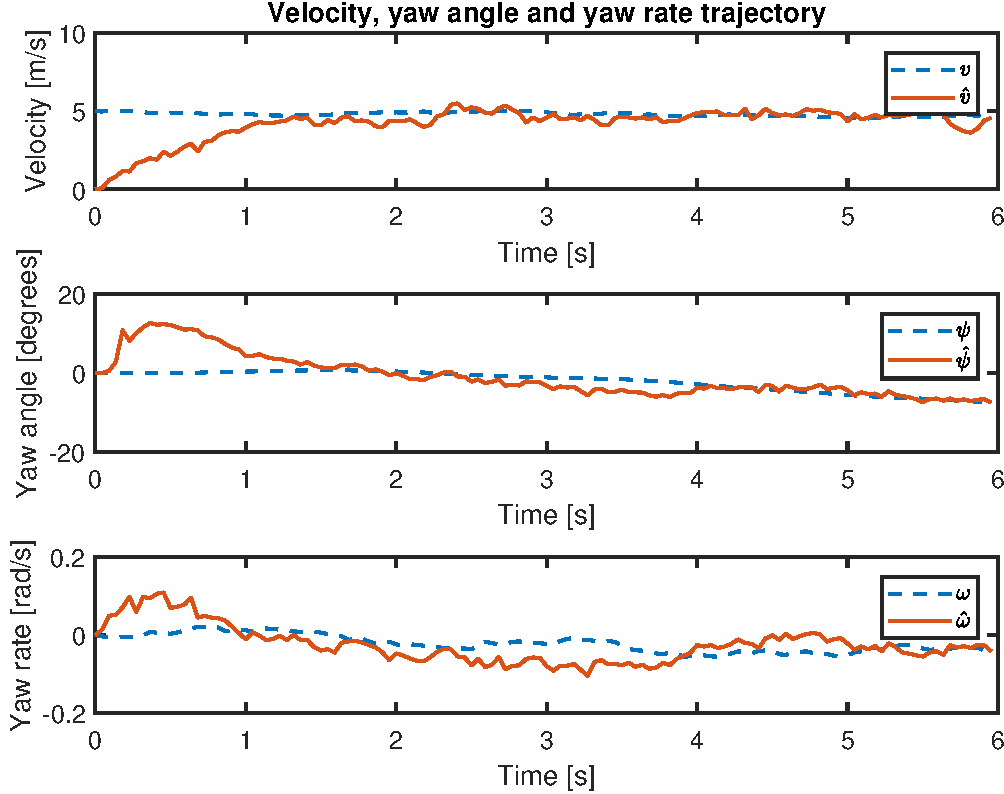
\includegraphics[width=\textwidth]{Traj/20_MC_TrajOther}
	\end{columns}
\end{frame}

\begin{frame}{Monte Carlo Results -- No. 1}
	\begin{columns}[T]
	\column{0.45\textwidth}
	\begin{figure}
		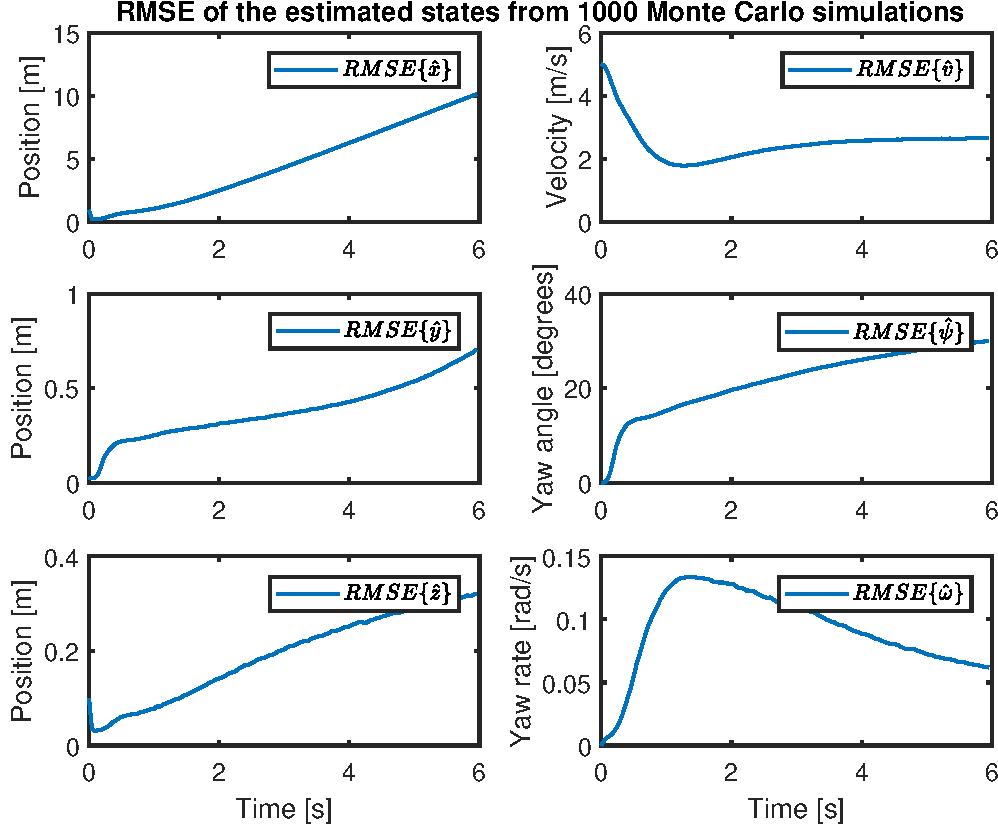
\includegraphics[width=\textwidth]{MC/27_MC_1000_Rmse}
		\caption{Only \roi measurements.}
	\end{figure}
	\column{0.45\textwidth}
	\begin{figure}
		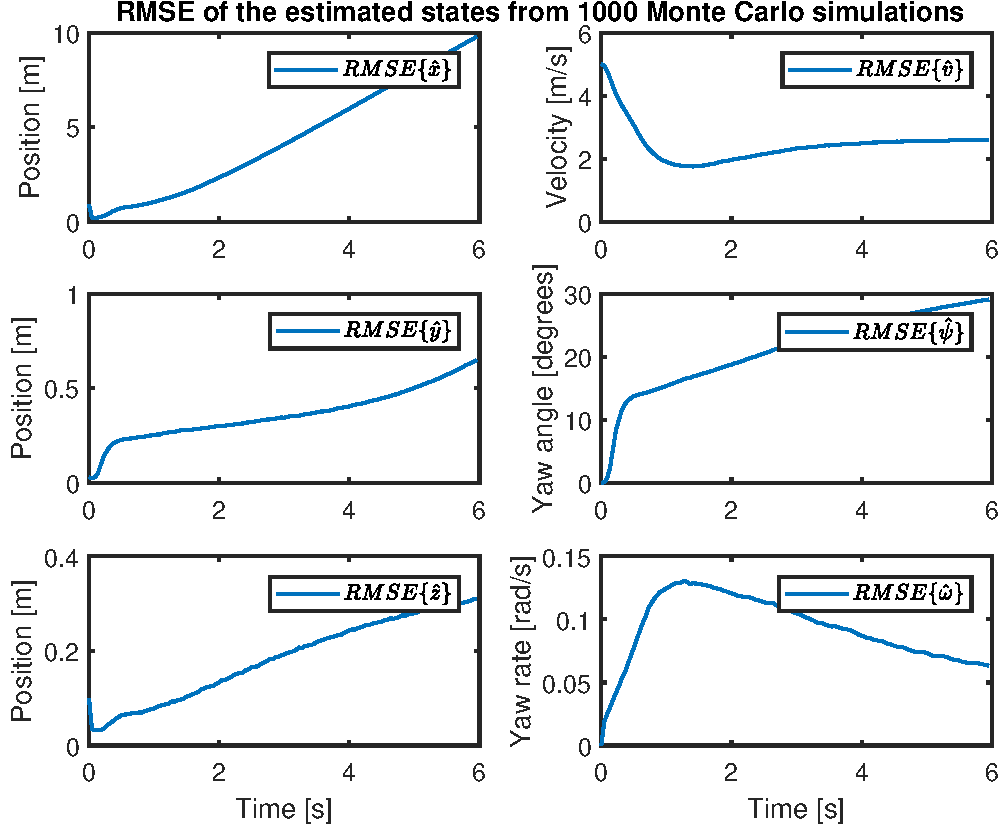
\includegraphics[width=\textwidth]{MC/22_MC_1000_Rmse}
		\caption{\roi and angular rate (with noise variance 1 rad/s) measurements.}
	\end{figure}
	\end{columns}
\end{frame}

\begin{frame}{Monte Carlo Results -- No. 1}
	\begin{columns}[T]
	\column{0.45\textwidth}
	\begin{figure}
		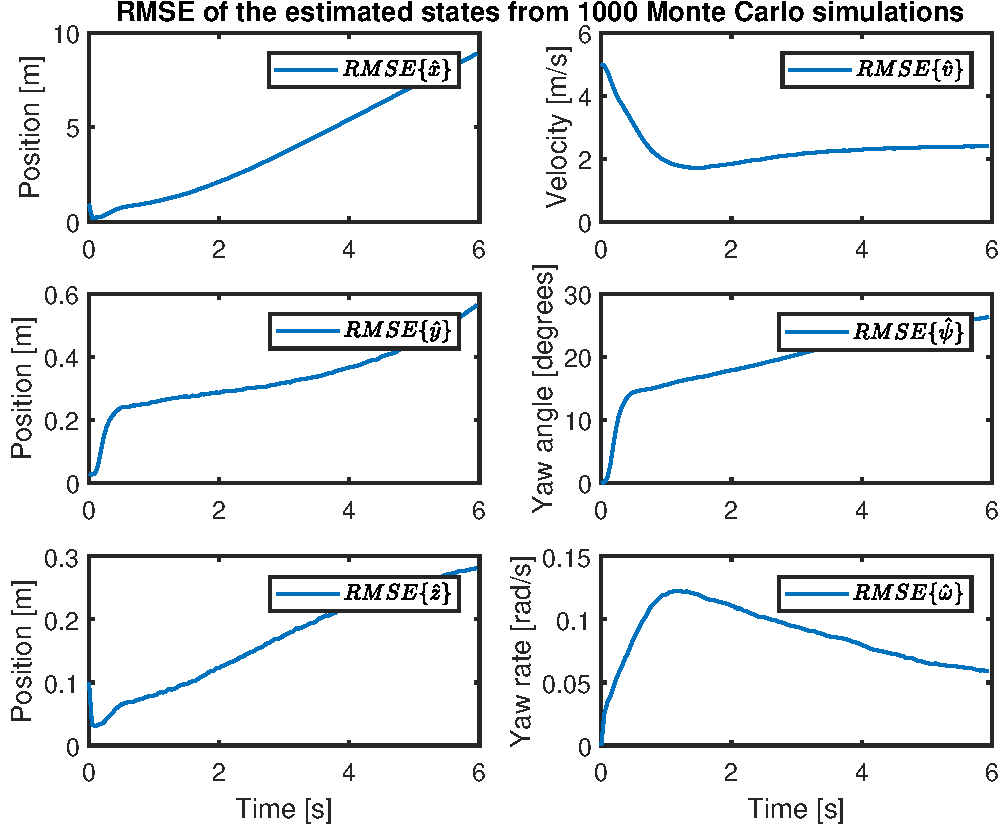
\includegraphics[width=\textwidth]{MC/21_MC_1000_Rmse}
		\caption{\roi and angular rate (with noise variance 0.5 rad/s) measurements.}
	\end{figure}
	\column{0.45\textwidth}
	\begin{figure}
		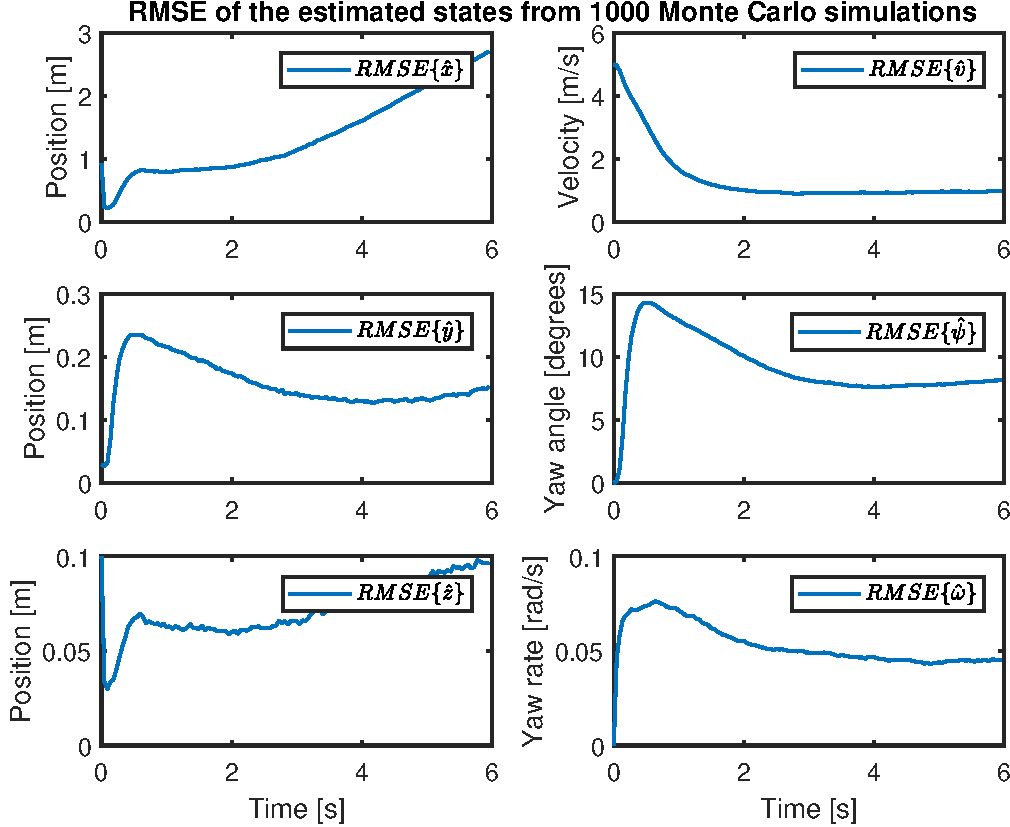
\includegraphics[width=\textwidth]{MC/20_MC_1000_Rmse}
		\caption{\roi and angular rate (with noise variance 0.1 rad/s) measurements.}
	\end{figure}
	\end{columns}
\end{frame}

\begin{frame}{Monte Carlo Simulations -- No. 2}
	The target is turning to the right.
	\vspace{1em}
	\begin{columns}
	\column{0.45\textwidth}
	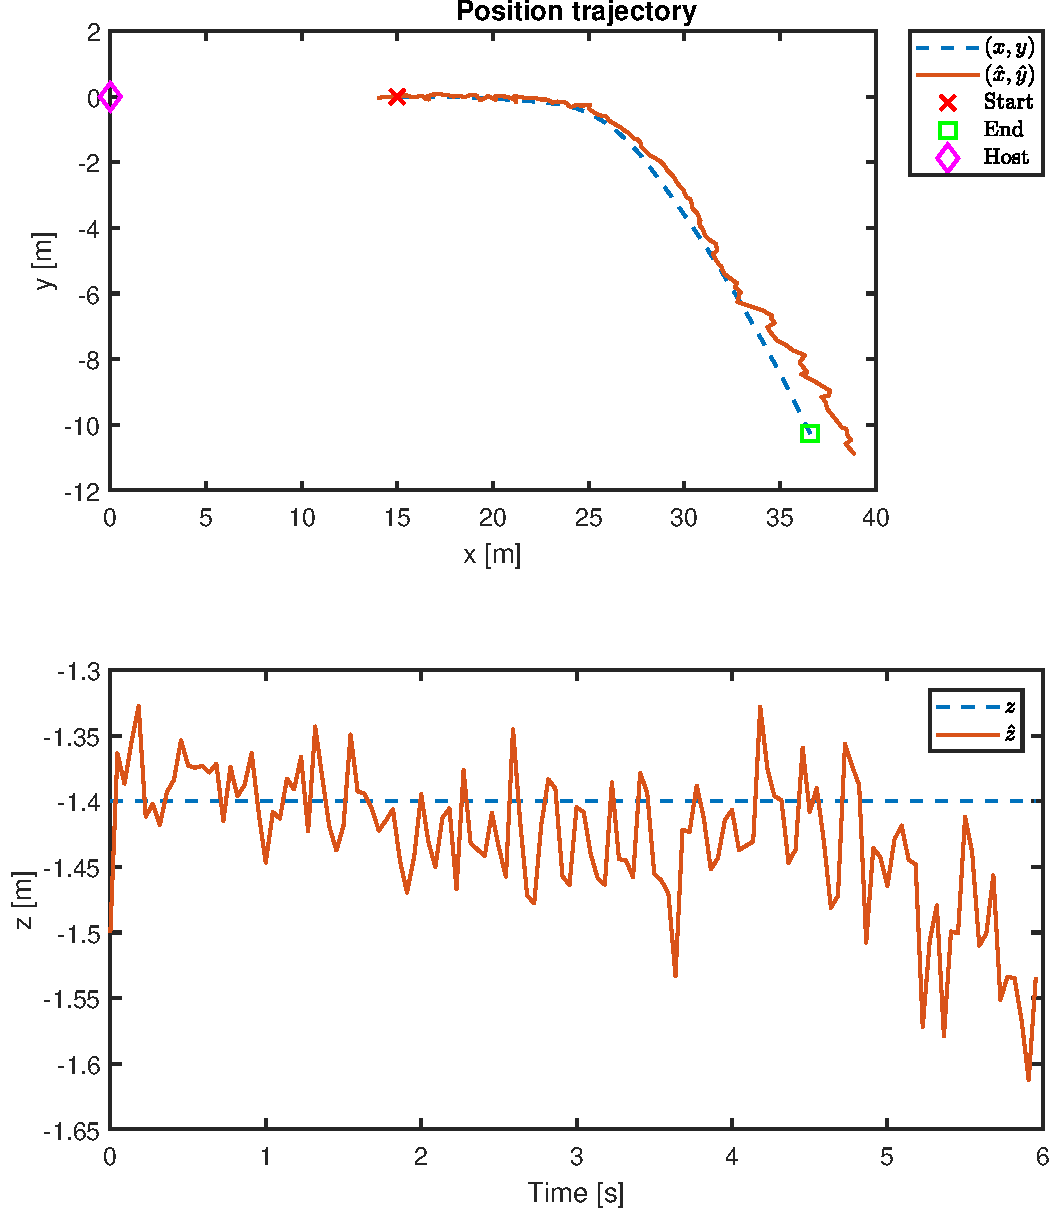
\includegraphics[width=\textwidth]{Traj/23_MC_TrajPos}
	\column{0.45\textwidth}
	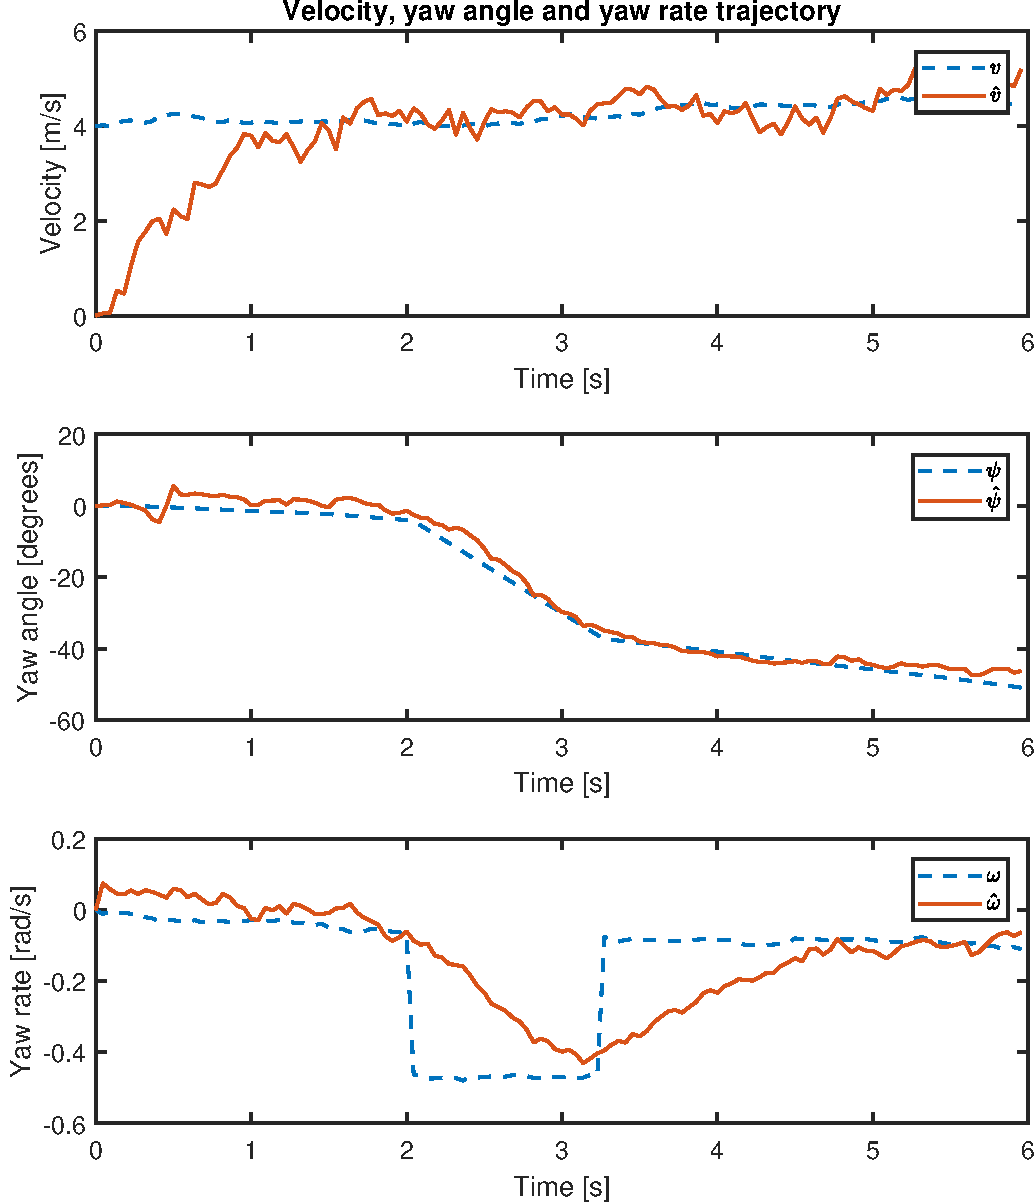
\includegraphics[width=\textwidth]{Traj/23_MC_TrajOther}
	\end{columns}
\end{frame}

\begin{frame}{Monte Carlo Results -- No. 2}
	\begin{columns}[T]
	\column{0.45\textwidth}
	\begin{figure}
		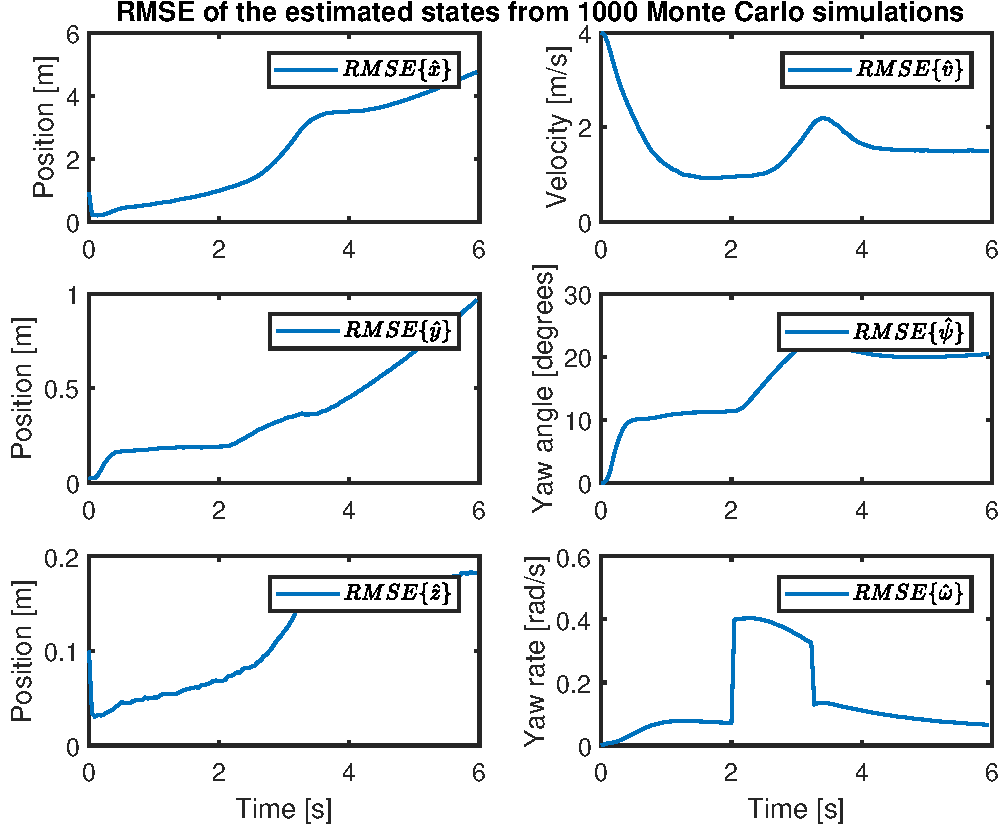
\includegraphics[width=\textwidth]{MC/13_MC_1000_Rmse}
		\caption{Only \roi measurements.}
	\end{figure}
	\column{0.45\textwidth}
	\begin{figure}
		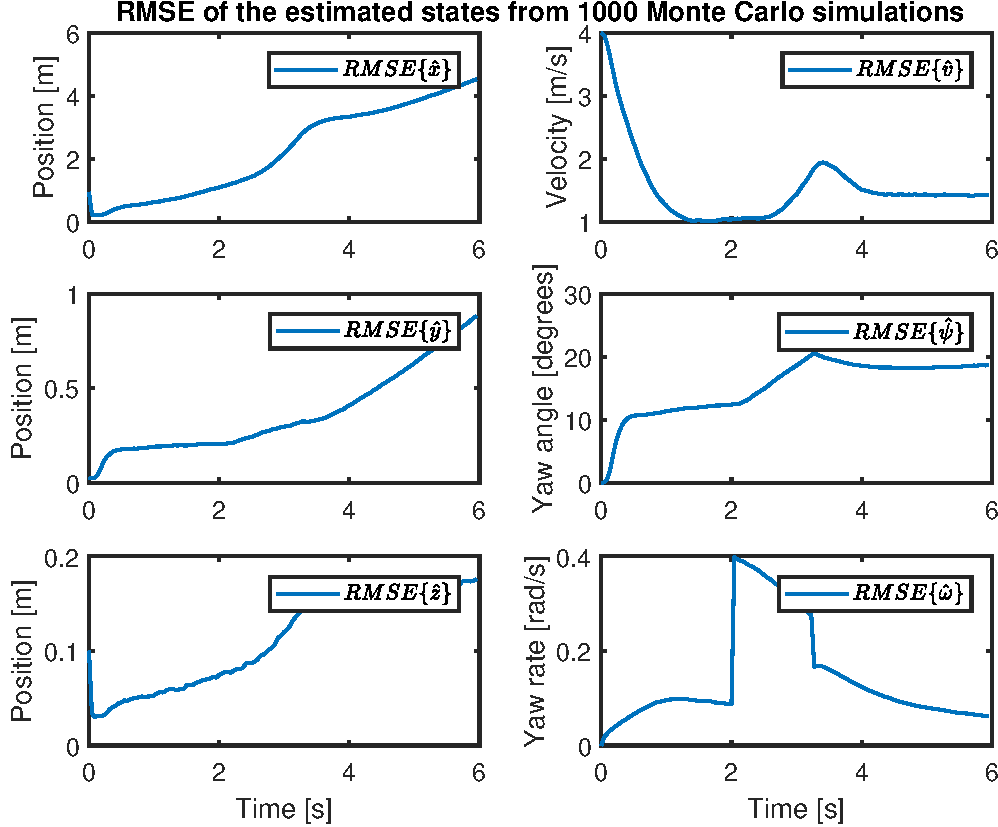
\includegraphics[width=\textwidth]{MC/25_MC_1000_Rmse}
		\caption{\roi and angular rate (with noise variance 1 rad/s) measurements.}
	\end{figure}
	\end{columns}
\end{frame}

\begin{frame}{Monte Carlo Results -- No. 2}
	\begin{columns}[T]
	\column{0.45\textwidth}
	\begin{figure}
		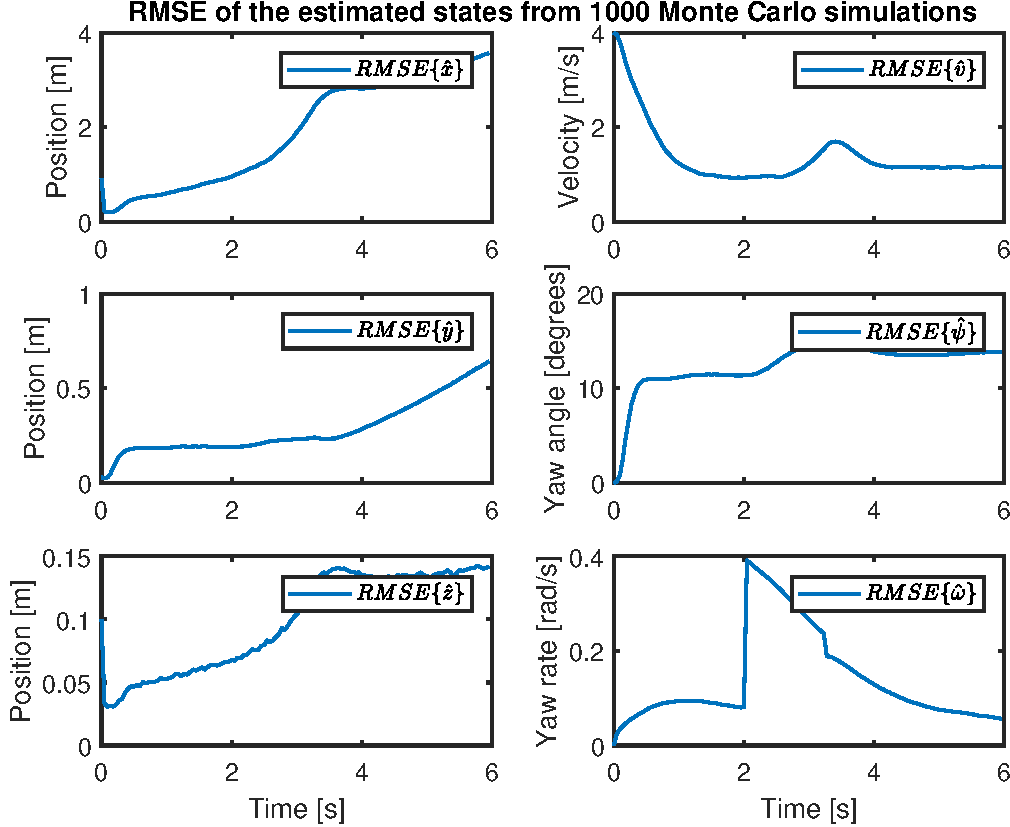
\includegraphics[width=\textwidth]{MC/24_MC_1000_Rmse}
		\caption{\roi and angular rate (with noise variance 0.5 rad/s) measurements.}
	\end{figure}
	\column{0.45\textwidth}
	\begin{figure}
		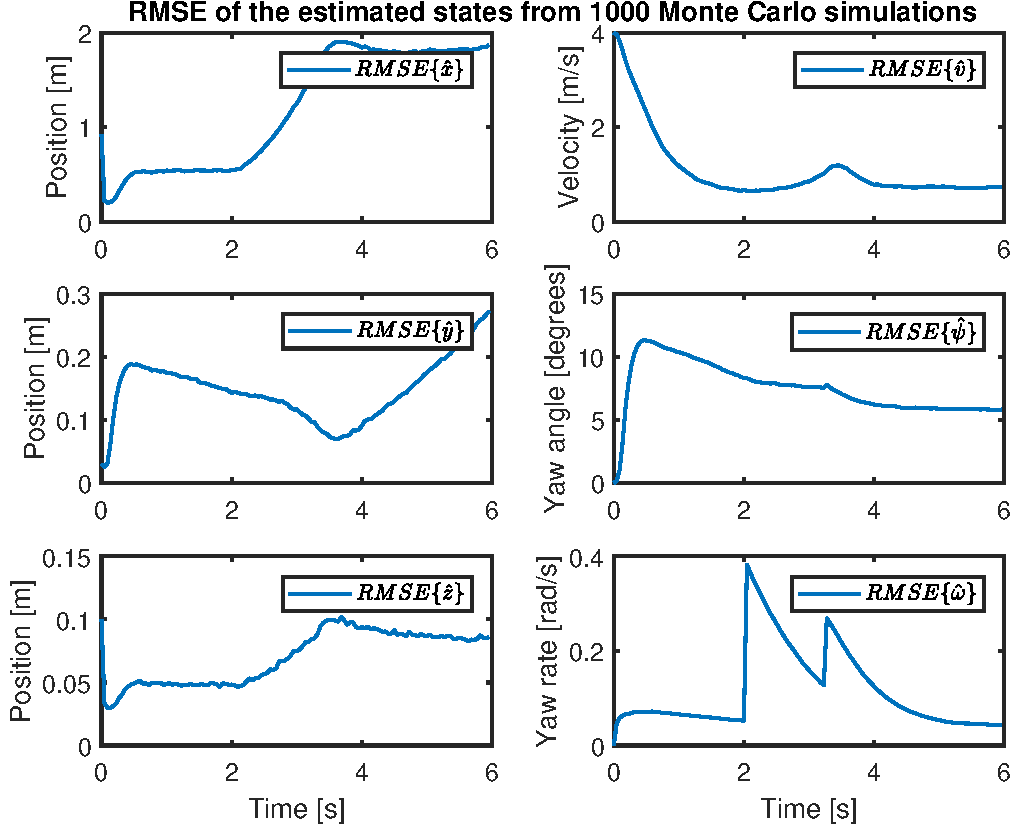
\includegraphics[width=\textwidth]{MC/23_MC_1000_Rmse}
		\caption{\roi and angular rate (with noise variance 0.1 rad/s) measurements.}
	\end{figure}
	\end{columns}
\end{frame}

\begin{frame}{Monte Carlo Results with Corner Measurements}
	\begin{columns}[T]
	\column{0.45\textwidth}
	Driving straight (no. 1):
	\begin{figure}
		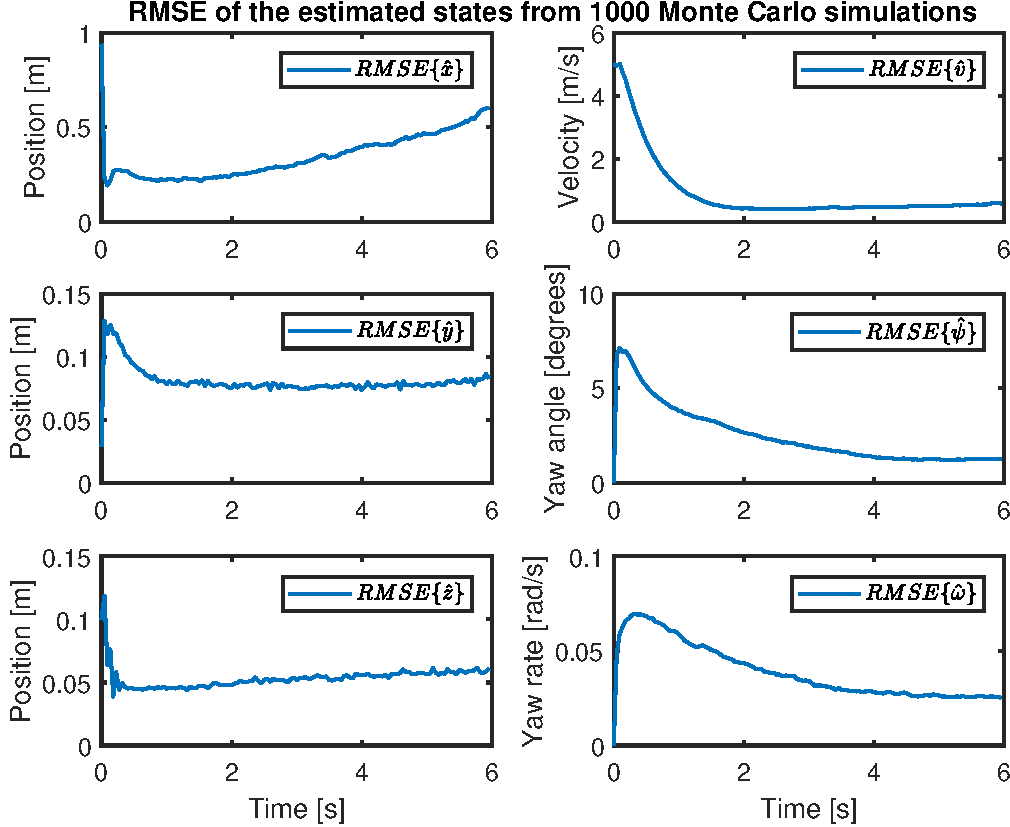
\includegraphics[width=\textwidth]{MC/30_MC_1000_Rmse}
		\caption{\roi, angular rate and corner measurements.}
	\end{figure}
	\column{0.45\textwidth}
	Turning right (no. 2):
	\begin{figure}
		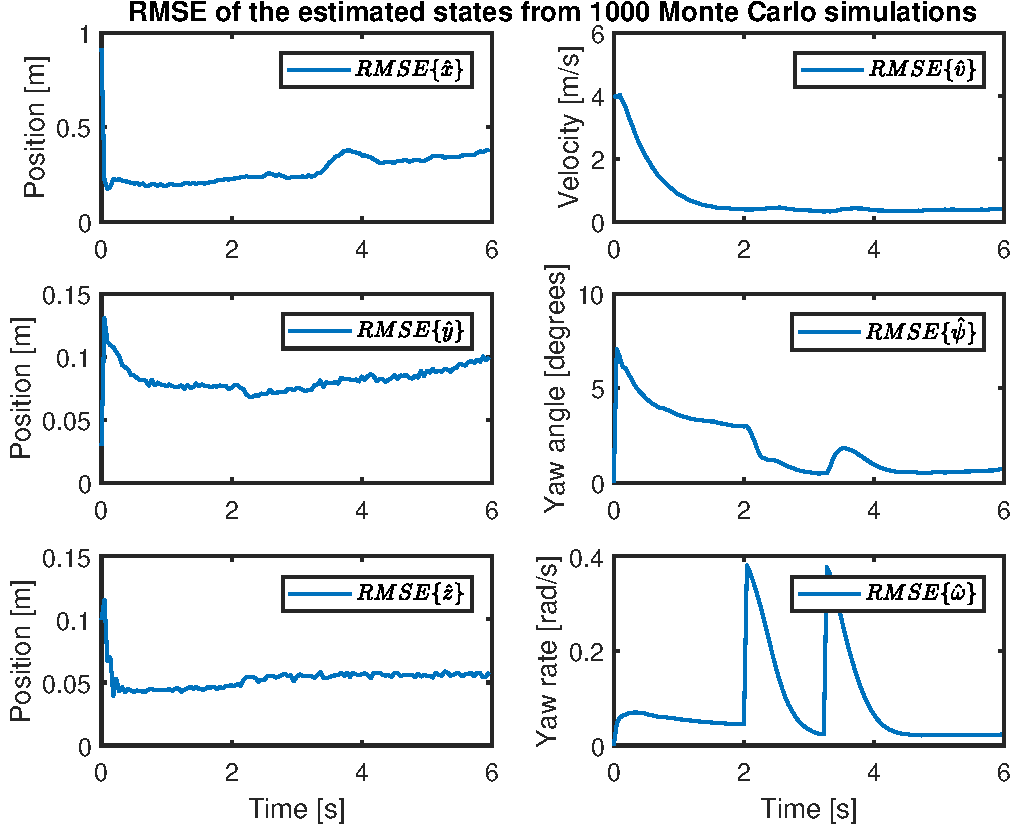
\includegraphics[width=\textwidth]{MC/29_MC_1000_Rmse}
		\caption{\roi, angular rate and corner measurements.}
	\end{figure}
	\end{columns}
\end{frame}

\subsection{Homography Estimation}

\begin{frame}{Homography Estimation Results -- Simulations}
	Simulation of a moving rectangle with different Gaussian noise realisations.
	\vspace{-2.5em}
	\begin{columns}[T]
	\column{0.45\textwidth}
	\begin{figure}
		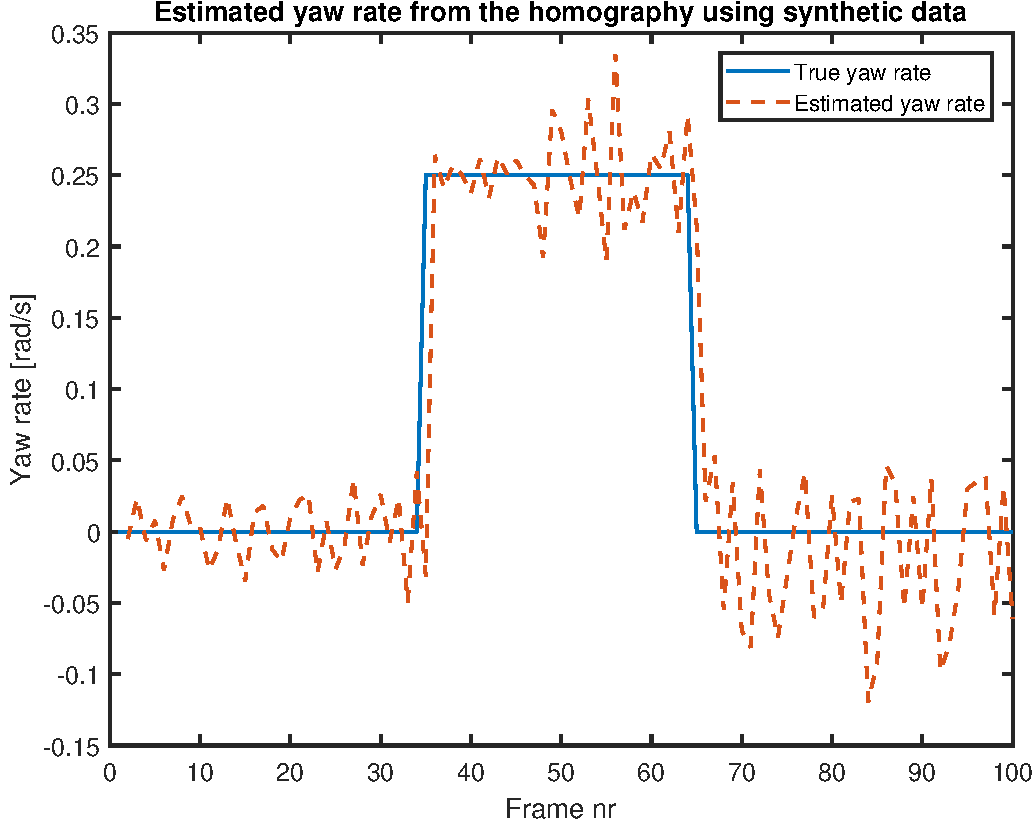
\includegraphics[height=0.375\textheight]{Hom/rect_1e-2}
		\vspace{-1.25em}
		\caption{Standard deviation 0.01 [px].}
	\end{figure}
	\vspace{-2.5em}
	\begin{figure}
		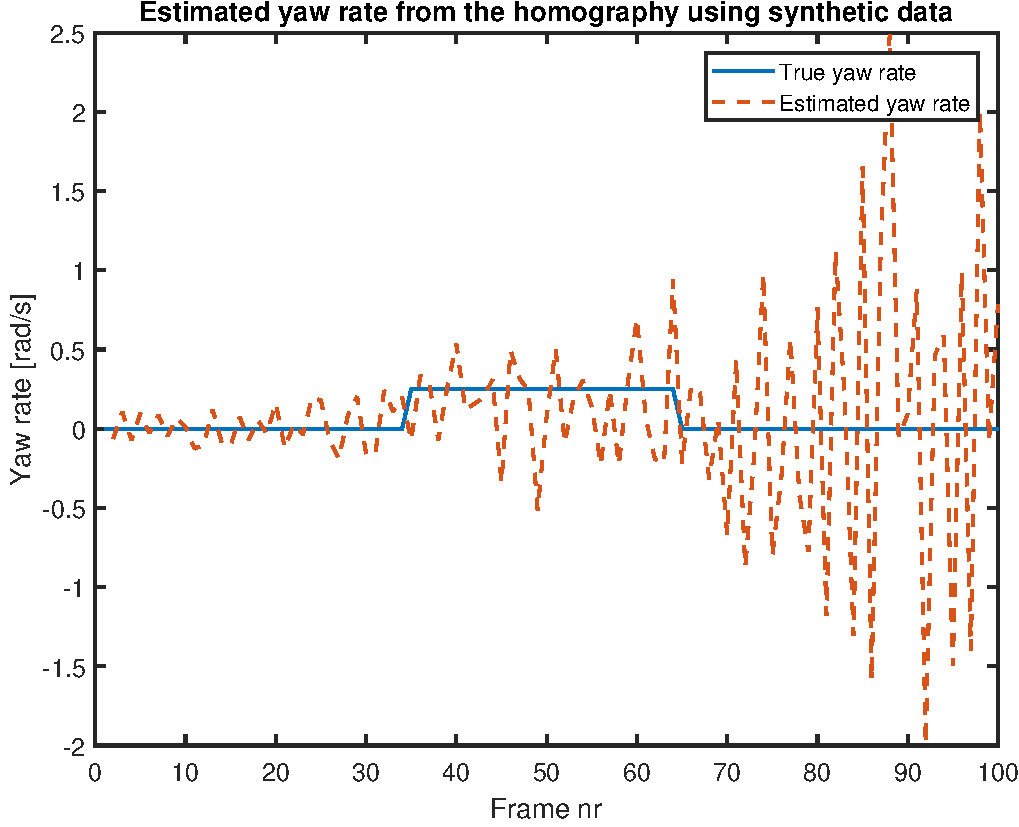
\includegraphics[height=0.375\textheight]{Hom/rect_1e-1}
		\vspace{-1.25em}
		\caption{Standard deviation 0.1 [px].}
	\end{figure}
	\column{0.45\textwidth}
	\begin{figure}
		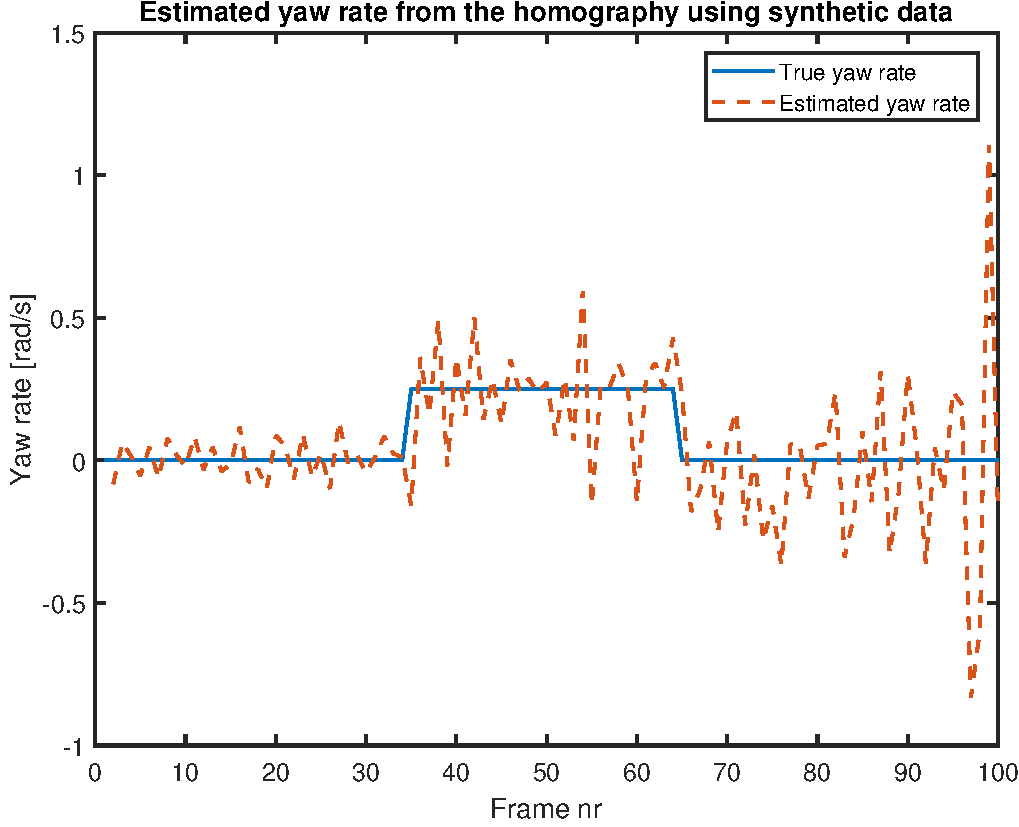
\includegraphics[height=0.375\textheight]{Hom/rect_5e-2}
		\vspace{-1.25em}
		\caption{Standard deviation 0.05 [px].}
	\end{figure}
	\vspace{-2.5em}
	\begin{figure}
		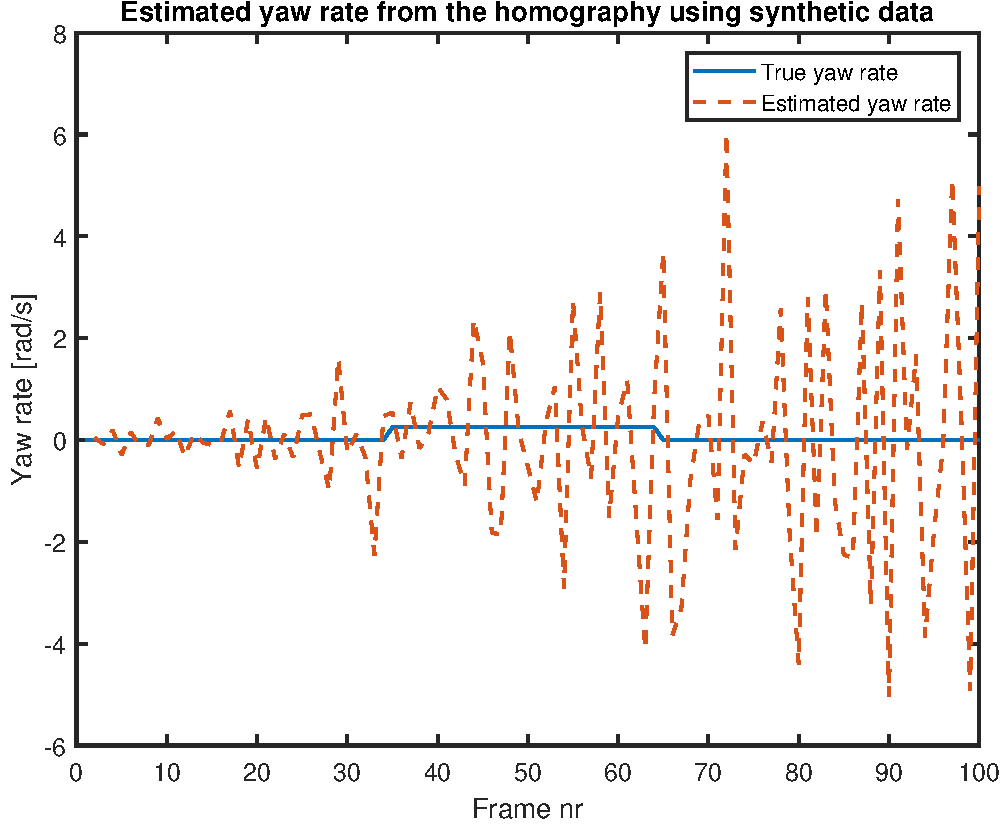
\includegraphics[height=0.375\textheight]{Hom/rect_5e-1}
		\vspace{-1.25em}
		\caption{Standard deviation 0.5 [px].}
	\end{figure}
	\end{columns}
\end{frame}

\begin{frame}{Homography Estimation Results -- Real-world Data}
	\begin{columns}[T]
	\column{0.45\textwidth}
	\begin{figure}
		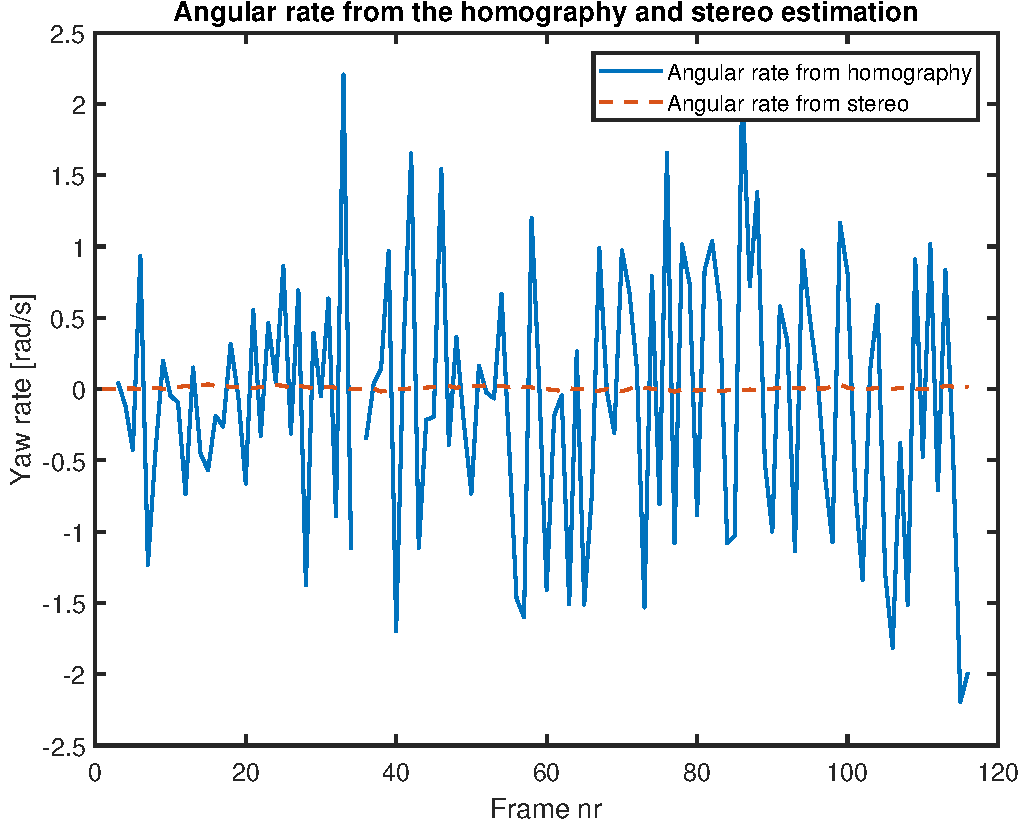
\includegraphics[width=\textwidth]{Hom/155532_AngVelComparison}
		\caption{Target driving straight and has a variance of 0.8 rad/s on the angular rate data.}
	\end{figure}
	\column{0.45\textwidth}
	\begin{figure}
		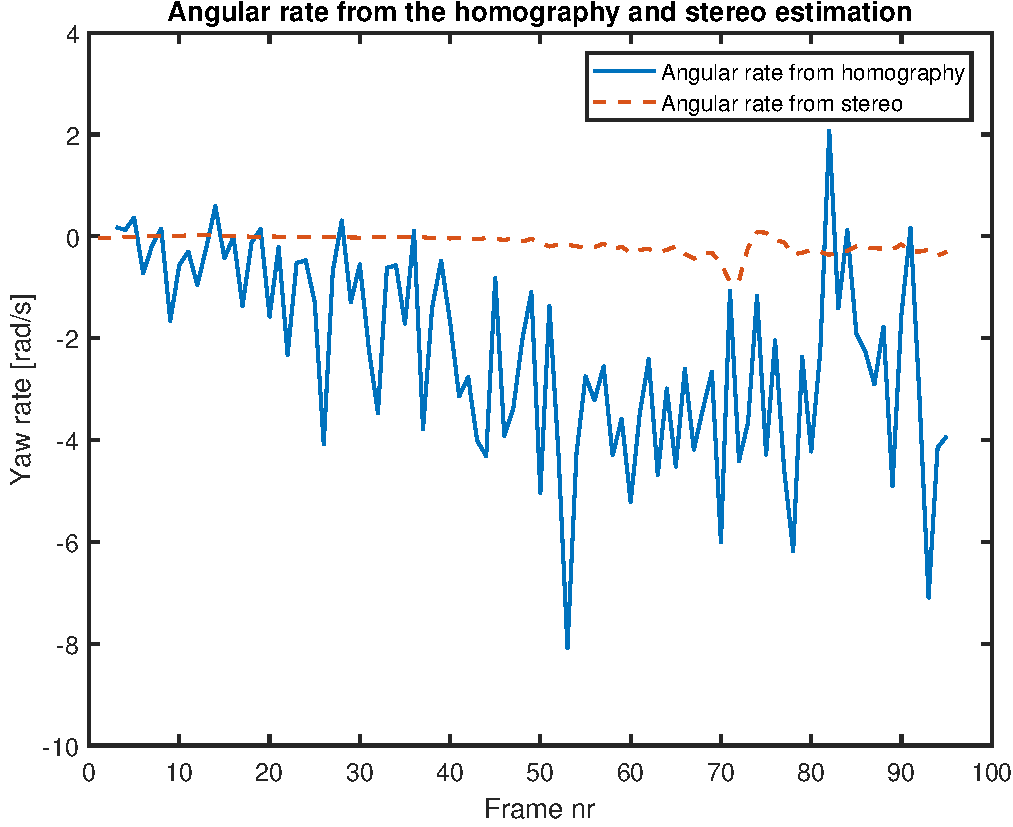
\includegraphics[width=\textwidth]{Hom/155733_AngVelComparison}
		\caption{Target turning right and has a variance of  2 rad/s on the angular rate data.}
	\end{figure}
	\end{columns}
\end{frame}

\subsection{Stereo Comparison}

\begin{frame}{Stereo Comparison -- No. 1}
	The target is driving straight.
	\begin{columns}[T]
	\column{0.45\textwidth}
	\begin{figure}
		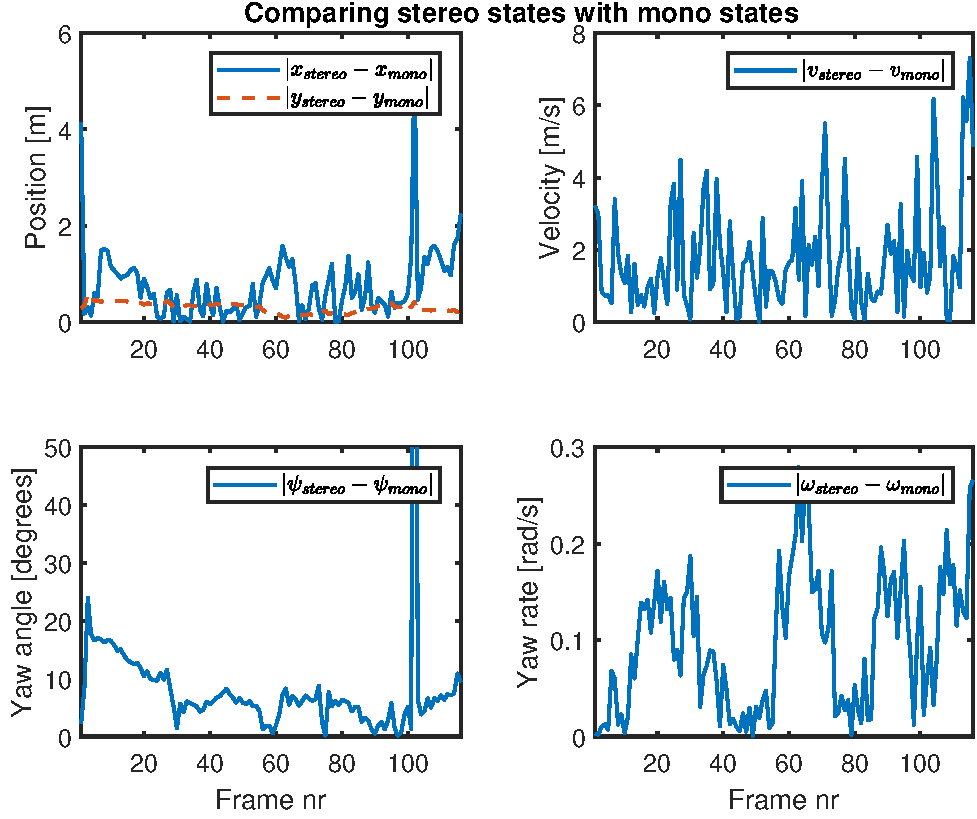
\includegraphics[width=\textwidth]{Stereo/155532_RoiAngVel_gate_klt}
		\caption{\roi and angular rate measurements.}
	\end{figure}
	\column{0.45\textwidth}
	\begin{figure}
		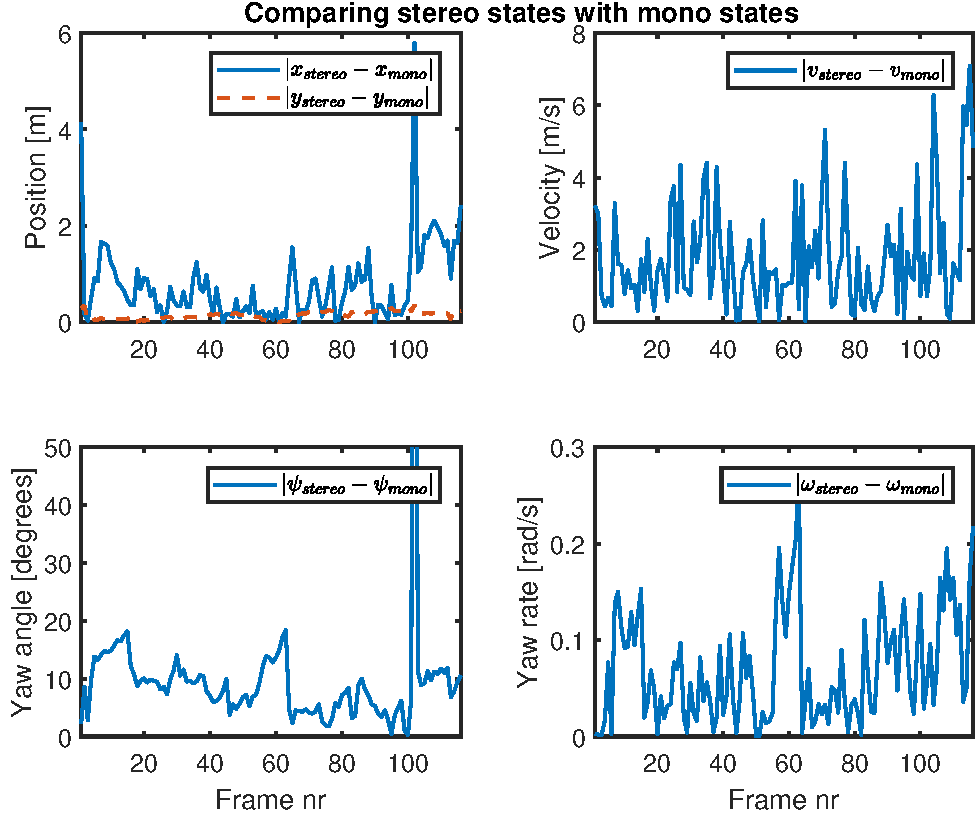
\includegraphics[width=\textwidth]{Stereo/155532_AllMeasurements_gate_klt}
		\caption{\roi, angular rate and corner measurements.}
	\end{figure}
	\end{columns}
\end{frame}

\begin{frame}{Stereo Comparison -- No. 2}
	The target is turning to the right.
	\begin{columns}[T]
	\column{0.45\textwidth}
	\begin{figure}
		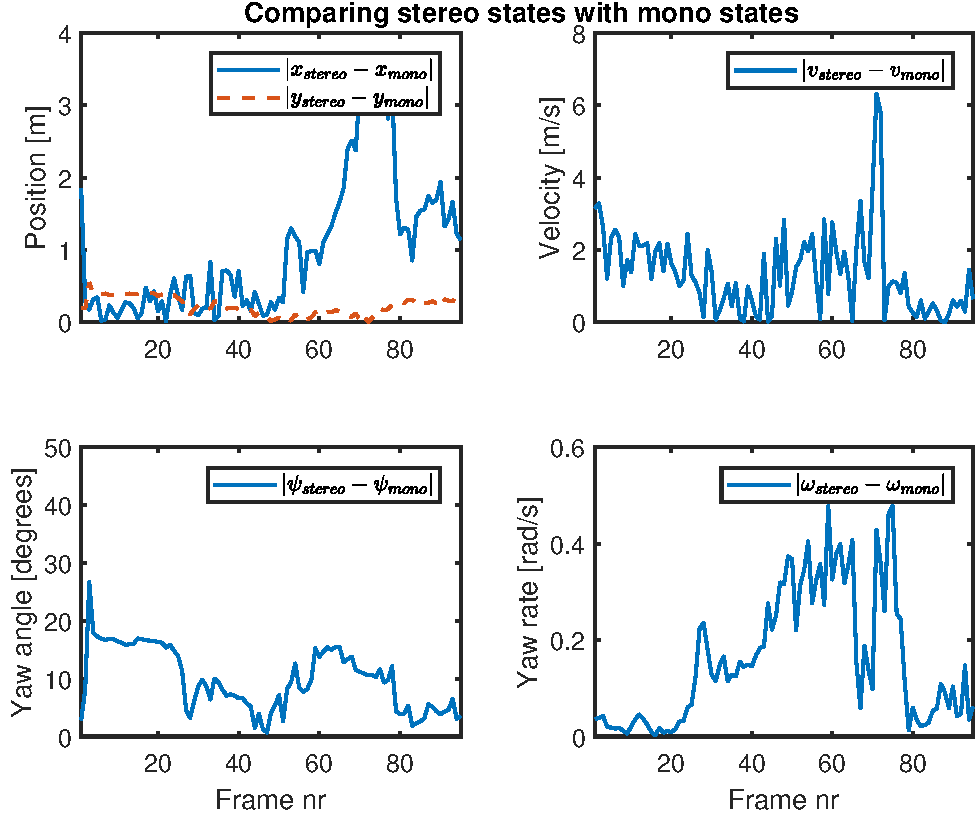
\includegraphics[width=\textwidth]{Stereo/155733_RoiAngVel_gate_klt}
		\caption{\roi and angular rate measurements.}
	\end{figure}
	\column{0.45\textwidth}
	\begin{figure}
		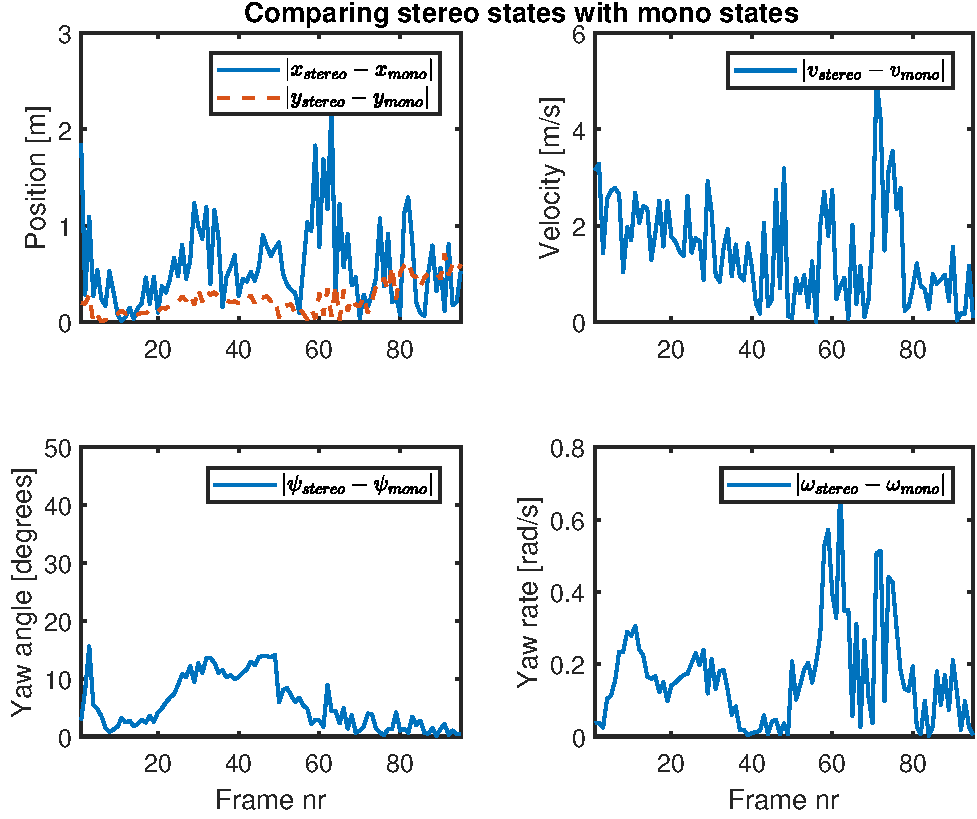
\includegraphics[width=\textwidth]{Stereo/155733_AllMeasurements_gate_klt_perf}
		\caption{\roi, angular rate and corner measurements.}
	\end{figure}
	\end{columns}
\end{frame}

% -------------------
\section{Conclusions}
% -------------------

\begin{frame}{Conclusions}
	\begin{itemize}
		\item The heading can be estimated
		\begin{itemize}
			\item given the proper measurements,
			\item with high enough accuracy.
		\end{itemize}
		\item The extended Kalman filter is a suitable filter structure.
		\item Still some performance difference compared to stereo.
	\end{itemize}
\end{frame}

\end{document}